\documentclass{cumcmthesis}

\usepackage[framemethod=TikZ]{mdframed}
\usepackage{url}
\usepackage{float}
\usepackage{array}
\usepackage{tabularx}
\usepackage{longtable}
\usepackage{subcaption}
\usepackage{listings}

\lstset{
    language=Python,
    basicstyle=\ttfamily\scriptsize,
    keywordstyle=\bfseries,
    commentstyle=\itshape,
    numbers=left,
    numberstyle=\tiny,
    stepnumber=1,
    numbersep=6pt,
    frame=single,
    breaklines=true,
    breakatwhitespace=false,
    columns=fullflexible,
    keepspaces=true,
    showstringspaces=false,
    xleftmargin=2em,
    framexleftmargin=1.5em
}
\renewcommand{\lstlistingname}{代码}

\graphicspath{{figures/}}

\newcommand{\kwh}{\mathrm{kWh}}
\newcommand{\yuan}{\text{元}}
\newcommand{\Tset}{\mathcal{T}}

\title{微网外部购电与储能调度优化研究}

\begin{document}

\maketitle

\begin{abstract}
\textbf{}本文的统一建模逻辑是先定义真实运行中的功率平衡，再把所有功率数据换算为十分钟电量，最后在同一储能状态方程和日循环边界下比较不同信息结构的调度策略。问题一提供确定性基准，问题二把历史预测误差转化为安全裕度，问题三利用新到达的光伏预报修正尚未执行的计划，问题四则进一步把日期--时段动态电价纳入目标函数。四问并非相互独立的四个算例，而是从“已知信息下的最优调度”逐步过渡到“信息不完全条件下的风险控制与反馈决策”。

\textbf{针对问题一：}将功率数据转换为十分钟电量，建立含供需平衡、储能效率、容量、功率和日循环约束的确定性线性规划。基准日结果显示，储能优化使购电费用由无储能方案的48052.05元降至35126.95元，下降26.90\%。

\textbf{针对问题二：}在每日0:00只使用前14天历史净负荷，采用经验均值和经验标准差构造安全净负荷，建立机会约束的日前模型，并用334天真实数据回测。固定安全系数$K=0.80$时，总成本为1654.76万元，紧急购电量为14.67万kWh。

\textbf{针对问题三：}对每天0:00、6:00、12:00和18:00发布的光伏预报进行跨日截断和线性插值，在计划偏差结算规则下建立MPC滚动模型。主方案$\beta=0.95$的总成本为1368.87万元，相对仅执行0:00计划节省8.03\%。

\textbf{针对问题四：}将基础分时电价替换为按日期和时段变化的动态电价，分别重算机会约束日前模型和MPC模型。4-2与4-3总成本分别为1740.24万元和1433.19万元；在相同4-3模型下，MPC相对0:00固定计划节省121.14万元，节省率为7.79\%。

在题目数据、日循环边界和本文回测口径下，储能跨时段转移、风险裕度和预测更新共同决定微网调度的经济性与供电可靠性。


\textbf{实验验证与结论：}为保证比较具有可解释性，本文将决策信息、物理执行和事后结算严格分开。问题二至问题四均使用2025年2月1日至12月31日的334天样本进行历史回放；计划阶段只使用对应时点可获得的数据，回测阶段才使用真实负荷和真实光伏。评价指标同时包含总成本、紧急购电量、紧急购电天数和弃光量，并通过无储能基准、固定计划基准、参数扫描和消融实验识别各模型机制的实际作用。结果显示，单纯增加保守程度可以降低部分紧急购电，但可能增加普通购电和弃光；适度预测折减与日内滚动更新在本数据集上取得了更好的成本--风险平衡。由于所有参数选择均基于同一历史样本，本文将结论限定为给定数据、费用规则和日循环假设下的实验结论，并在文末讨论跨日SOC传递、价格预测和独立测试期等进一步工作。

\keywords{微网调度\quad 储能优化\quad 机会约束\quad 模型预测控制\quad 动态电价}
\end{abstract}

\section{引言}

\subsection{问题背景}

微网由负荷、光伏、储能和外部电网构成。题目数据覆盖基础电价、全年负荷与实际光伏、分时光伏预测及动态电价；每日至少划分为144个十分钟时段。储能容量、功率上限、效率和SOC边界决定跨时段调度的可行域，预测误差和偏差结算决定日前计划的实际成本。本文将经济性、光伏消纳和供电风险统一纳入购电—储能—结算模型\cite{olivares2014}。

调度问题同时具有时间耦合和信息不完全特征。储能能够转移低价或光伏富余电量，但设备边界限制了转移规模；日前计划只能使用决策时信息，真实负荷与光伏偏差可能产生紧急购电或弃光。因此，本文在统一物理约束下分别评价计划成本、执行轨迹和真实结算成本。

\subsection{问题重述}

四个问题具有清晰的递进关系：问题一假定全天负荷和光伏预测已知，求确定性日前计划；问题二只在每日0:00使用历史信息制定计划，并用实际数据评价紧急购电风险；问题三在新的光伏预测到达后滚动调整尚未执行的计划；问题四进一步考虑电价随日期和时段变化的情形，并分别完成机会约束日前优化和动态电价MPC调整。

\section{总体分析}

本文按“确定性基准—不确定性控制—预测反馈—动态价格扩展”推进。四问均以十分钟电量为决策单位，统一采用储能状态方程和日循环边界；计划阶段只使用当时可获得的信息，回测阶段才代入真实负荷和光伏。无储能对照、$K$扫描、MPC固定计划对照和$\beta$敏感性分别用于识别储能收益、风险—成本权衡、预测更新收益和保守程度影响\cite{boyd2004}。

\section{模型假设}

\subsection{基本假设}

为突出购电计划和储能调度的主要矛盾，作如下假设：
\begin{enumerate}
    \item 所有功率数据在十分钟时段内按常值处理，功率与电量通过式（2）换算；
    \item 光伏优先供给本地负荷，不能被负荷或储能吸收的富余光伏不向外网反送，计为弃光；
    \item 储能充放电效率恒定为0.9，且不设置同一时段同时充放电的额外二进制变量；正电价和效率损耗下，线性规划最优解通常不会主动安排这种无效循环；
    \item 问题二和4-2的净负荷统计仅使用目标日之前14天的历史样本；问题三和4-3的滚动优化仅使用对应发布时间已经获得的预测；
    \item 问题三沿用问题二的紧急购电5倍电价口径，以便三层费用可以在同一回测框架内比较；
    \item 每日采用始末储电量均为6000 kWh的闭环边界，因而回测结果用于逐日比较，不代表全年连续运行状态。
\end{enumerate}

\subsection{数据预处理与统一量纲}

记日内时段集合为$\Tset=\{0,1,\ldots,143\}$，单个时段长度为
\begin{equation}
    \Delta t=\frac{10}{60}=\frac{1}{6}\ \mathrm{h}.
    \tag{1}
\end{equation}
若输入的负荷功率和光伏功率分别为$P_{\mathrm{load},d,t}$和$P_{\mathrm{pv},d,t}$，则对应的时段电量为
\begin{equation}
    E_{\mathrm{load},d,t}=P_{\mathrm{load},d,t}\Delta t,qquad
    E_{\mathrm{pv},d,t}=P_{\mathrm{pv},d,t}\Delta t.
    \tag{2}
\end{equation}
定义实际净负荷为
\begin{equation}
    N_{d,t}=E_{\mathrm{load},d,t}-E_{\mathrm{pv},d,t}.
    \tag{3}
\end{equation}

\subsection{统一设备约束}

记$E_{\mathrm{ch},d,t}$和$E_{\mathrm{dis},d,t}$为储能充电量和放电量，$S_{d,t}$为时段边界处的储电量。储能状态满足
\begin{equation}
S_{d,t+1}=S_{d,t}+\eta_{\mathrm{ch}}E_{\mathrm{ch},d,t}
-\frac{E_{\mathrm{dis},d,t}}{\eta_{\mathrm{dis}}},
\qquad \eta_{\mathrm{ch}}=\eta_{\mathrm{dis}}=0.9.
\tag{4}
\end{equation}
单个十分钟时段的充放电上限为
\begin{equation}
0\leq E_{\mathrm{ch},d,t},E_{\mathrm{dis},d,t}
\leq E_{\max}=5000\Delta t=833.3333\ \kwh,
\tag{5}
\end{equation}
并满足
\begin{equation}
1200\leq S_{d,t}\leq10800,\qquad S_{d,0}=S_{d,144}=6000.
\tag{6}
\end{equation}
本文不考虑向外部电网反向售电，因此所有普通购电量均非负。

\section{符号说明}

\begin{table}[H]
\centering
\renewcommand\arraystretch{1.2}
\caption{统一符号说明}
\label{tab:symbols}
\begin{tabular}{p{3.5cm}p{7.3cm}p{2.0cm}}
\toprule
\textbf{符号} & \textbf{含义} & \textbf{单位}\\
\midrule
$d,t$ & 日期和十分钟时段索引 & --\\
$C_{d,t}$、$p_t$ & 动态电价和基础分时电价 & 元/kWh\\
$E_{\mathrm{grid},d,t}$ & 外部电网普通购电量 & kWh\\
$E^0_{d,t}$、$E_{d,t}$ & 0:00原始计划和滚动调整后的购电量 & kWh\\
$E_{\mathrm{load},d,t}$、$E_{\mathrm{pv},d,t}$ & 负荷电量和实际光伏电量 & kWh\\
$\widehat E^{(r)}_{\mathrm{pv},d,t}$ & 发布时刻$r$形成的光伏预测电量 & kWh\\
$E_{\mathrm{emer},d,t}$、$E_{\mathrm{curt},d,t}$ & 紧急购电量和弃光量 & kWh\\
$u^+_{d,t}$、$u^-_{d,t}$ & 增购量和退订量辅助变量 & kWh\\
$K$、$\varepsilon$、$\beta$ & 安全裕度、机会约束违约概率、问题三和问题四共用的预测折减系数 & --\\
\bottomrule
\end{tabular}
\end{table}

\section{模型的建立与求解}

\subsection{统一实验口径}

问题一使用题目指定的单日数据；问题二至问题四回测2025年2月1日至12月31日的334天样本。问题二采用前14天净负荷经验均值和分母为$W$的标准差，4-2沿用同一窗口但使用分母为$W-1$的标准差，具体口径与对应程序一致。各日优化均满足$S_{d,0}=S_{d,144}=6000$，因此结果用于逐日比较，不代表全年连续SOC轨迹。

每个方案均按“决策—执行—结算”顺序评价：计划阶段仅使用决策时信息；回测阶段代入真实负荷、实际光伏和对应电价，计算普通购电、偏差费用、紧急购电及弃光。总成本$Z$为经济性指标，$Q_{\mathrm{emer}}$和$D_{\mathrm{emer}}$衡量供电风险，$Q_{\mathrm{curt}}$衡量光伏消纳损失。

\begin{table}[H]
\centering
\normalsize
\renewcommand\arraystretch{1.25}
\caption{四个问题的决策信息、模型和实验目的}
\label{tab:research_design}
\begin{tabularx}{\textwidth}{p{0.8cm}p{4.0cm}p{4.0cm}X}
\toprule
\textbf{问题} & \textbf{可用信息} & \textbf{模型} & \textbf{验证重点}\\
\midrule
1 & 单日电价、负荷和光伏预测 & 确定性线性规划 & 无储能对照，检验储能经济性与可行性\\
2 & 0:00前14天历史数据 & 机会约束日前规划 & 扫描$K$，分析常规购电与紧急购电的权衡\\
3 & 0:00、6:00、12:00、18:00光伏预报 & MPC滚动规划 & 固定0:00计划对照，检验预测更新收益\\
4 & 问题二、三信息与动态电价 & 动态电价机会约束与MPC & 区分价格与滚动修正作用，检验$K,\beta$敏感性\\
\bottomrule
\end{tabularx}
\end{table}

定义回测期内的总成本、紧急购电天数、紧急购电量和弃光量为
\begin{equation}
\begin{aligned}
Z&=\sum_d(C_{\mathrm{buy},d}+C_{\mathrm{dev},d}+C_{\mathrm{emer},d}),\\
D_{\mathrm{emer}}&=\sum_d\mathbf{1}\left(\sum_tE_{\mathrm{emer},d,t}>10^{-4}\right),\\
Q_{\mathrm{emer}}&=\sum_{d,t}E_{\mathrm{emer},d,t},\qquad
Q_{\mathrm{curt}}=\sum_{d,t}E_{\mathrm{curt},d,t}.
\end{aligned}
\tag{7a}
\end{equation}
其中，$C_{\mathrm{dev},d}$在问题一、问题二和4-2中为零；问题三和4-3按照题目偏差规则结算。比较策略时，以总成本作为经济性主指标，以$Q_{\mathrm{emer}}$和$D_{\mathrm{emer}}$描述供电风险，以$Q_{\mathrm{curt}}$描述光伏消纳损失。

\subsection{问题一的模型建立与求解：确定性日前购电与储能优化}

\subsubsection{具体分析}

问题一是全文的确定性基准。已知单日基础电价、负荷和光伏预测，将功率换算为十分钟电量，以购电费用最小为目标联合优化购电、充电、放电和SOC。模型包含供需平衡、效率、功率、容量及日循环约束。HiGHS求得基准日费用35126.95元，较无储能方案的48052.05元下降26.90%；容量、效率和影子价格实验用于检验该结论的物理与经济一致性。

\subsubsection{模型准备}

\paragraph{1. 数据预处理}

问题一使用题目给定的单日负荷、光伏预测和基础分时电价。程序将功率统一乘以$1/6$转换为十分钟电量，并按照$t=0,1,\ldots,143$建立全天离散时段。储能初始电量为$6000\kwh$，上下界为$1200$--$10800\kwh$，充放电效率均为$0.90$，单时段充放电上限为$4500\kwh$。已知输入为$(p_t,E_{\mathrm{load},t},E_{\mathrm{pv},t})$，决策变量为$(E_{\mathrm{grid},t},E_{\mathrm{ch},t},E_{\mathrm{dis},t})$，状态变量为$S_t$。

\paragraph{2. 算法选择}

本问的决策变量为连续电量，目标函数和供需平衡、储能递推、容量边界均为线性关系，因此选择线性规划。该方法能够直接处理$144$个时段的跨期耦合约束，并在给定数据下获得全局最优解；同时便于开展无储能对照、容量敏感性和效率敏感性实验。

\subsubsection{模型建立}

在全天负荷、光伏预测和电价均已知时，令$E_{\mathrm{grid},t}$为普通购电量。目标函数只计普通购电费用，因为问题一不含预测偏差和紧急购电结算：
\begin{equation}
\min Z_1=\sum_{t\in\Tset}p_tE_{\mathrm{grid},t}.
\tag{7}
\end{equation}
供需约束为
\begin{equation}
E_{\mathrm{grid},t}+E_{\mathrm{pv},t}+E_{\mathrm{dis},t}
\geq E_{\mathrm{load},t}+E_{\mathrm{ch},t},\qquad t\in\Tset.
\tag{8}
\end{equation}
式（8）的不等式允许右侧未被负荷或储能吸收的光伏自然弃光；在不允许反送电且弃光不计入目标时，引入弃光变量并写成等式与当前写法等价。式（4）描述充放电效率造成的SOC跨期耦合，式（5）限制设备功率，式（6）限制容量并固定日初、日末SOC。因正电价和效率损耗均为正，模型不会通过同时充放电获得目标值下降；日循环边界则排除了透支期末SOC的虚假收益。

\paragraph{模型性质与约束含义}
因此，在给定输入下问题一是标准连续线性规划；其可行域为线性约束定义的有界集合，采用HiGHS可直接获得全局最优解。储能只有在低价购电或光伏富余带来的未来收益能够覆盖效率损失时才产生充电动作，放电则优先服务于高价或光伏不足时段。

\subsubsection{模型求解}

求解流程为“读取144个时段数据—构造目标函数和约束矩阵—调用HiGHS—输出购电、充放电及SOC轨迹—检查SOC边界和日循环—与无储能基准比较”。HiGHS求得全天购电量59482.70 kWh、费用35126.95元；储能累计充电20740.67 kWh、放电16799.94 kWh，期末SOC回到6000 kWh。

\begin{table}[H]
\centering
\renewcommand\arraystretch{1.2}
\caption{问题一代表时段购电量与全天汇总}
\label{tab:q1result}
\begin{tabular}{lr}
\toprule
\textbf{时段或指标} & \textbf{购电量或费用}\\
\midrule
10:00--10:10 & 0.0000 kWh\\
12:00--12:10 & 486.4029 kWh\\
14:00--14:10 & 0.0000 kWh\\
16:00--16:10 & 394.9315 kWh\\
18:00--18:10 & 636.9826 kWh\\
20:00--20:10 & 0.0000 kWh\\
全天购电量 & 59482.6987 kWh\\
全天购电费 & 35126.9500 元\\
\bottomrule
\end{tabular}
\end{table}

图~\ref{fig:q1dispatch}和图~\ref{fig:q1soc}共同表明，储能在低价或光伏富余时段充电，在高价或光伏不足时段放电；SOC始终位于1200--10800 kWh且首尾相接。与无储能基准相比，费用减少
\begin{equation}
48052.05-35126.95=12925.10\ \text{元},
\tag{9}
\end{equation}
降幅为26.90\%，说明储能跨时段转移在该基准日具有可量化的经济收益。

\begin{figure}[H]
\centering
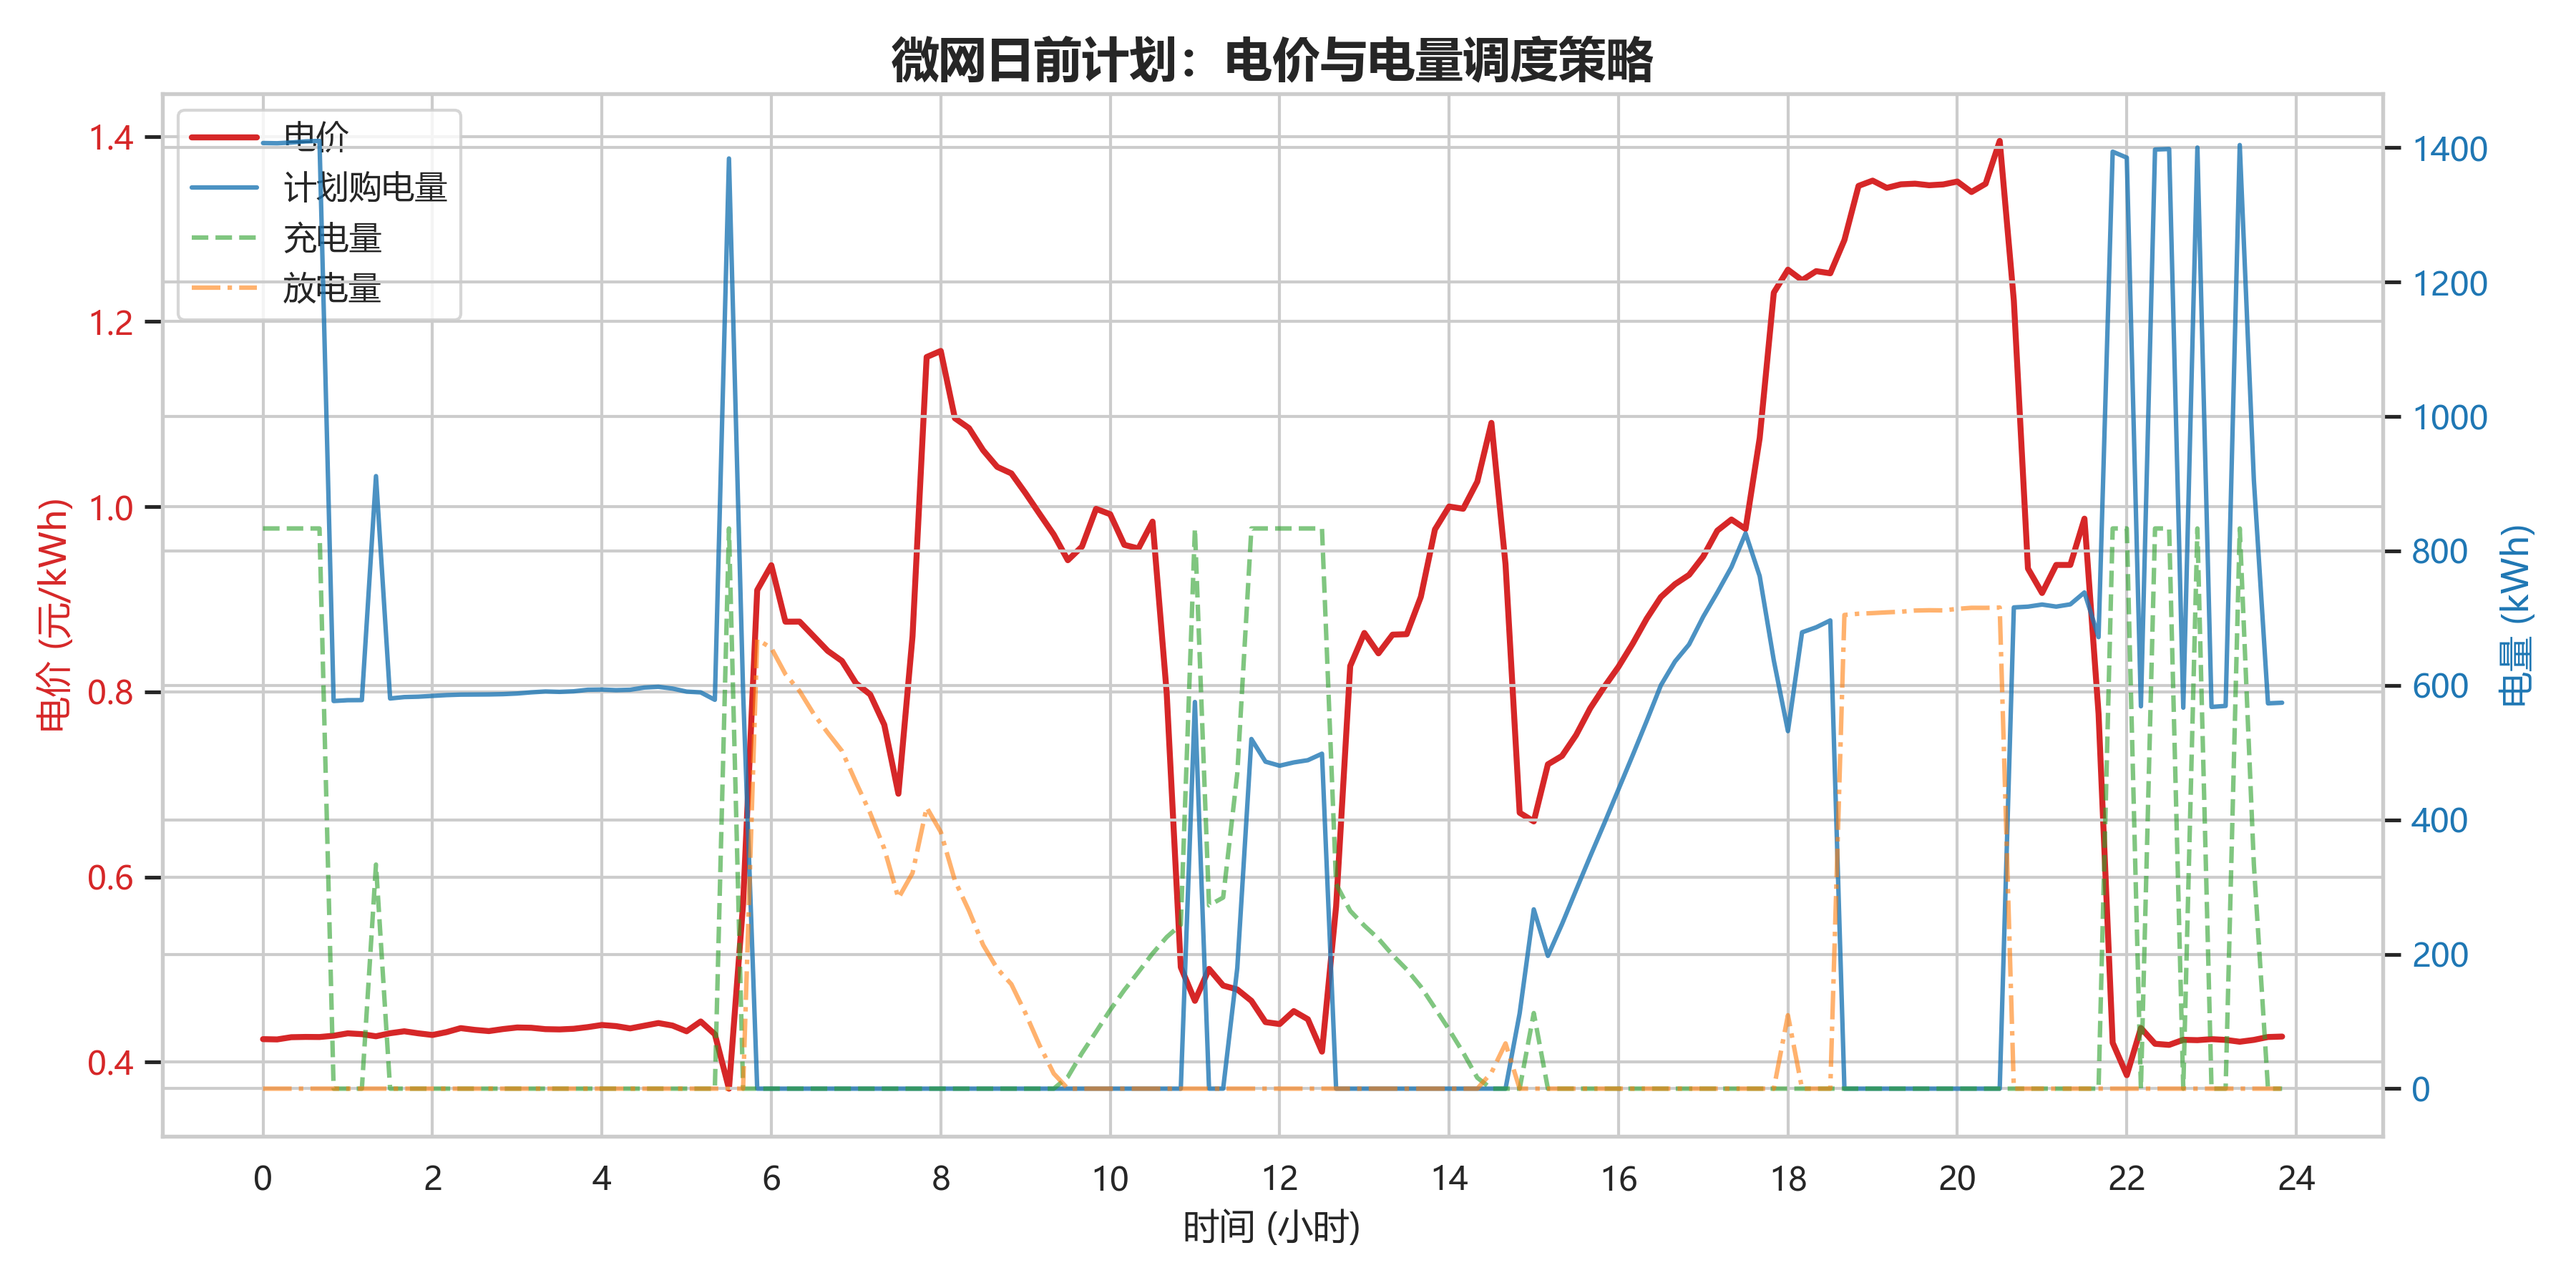
\includegraphics[width=.95\textwidth]{q1_dispatch.png}
\caption{问题一电价与购电、储能调度}
\label{fig:q1dispatch}
\end{figure}

\begin{figure}[H]
\centering
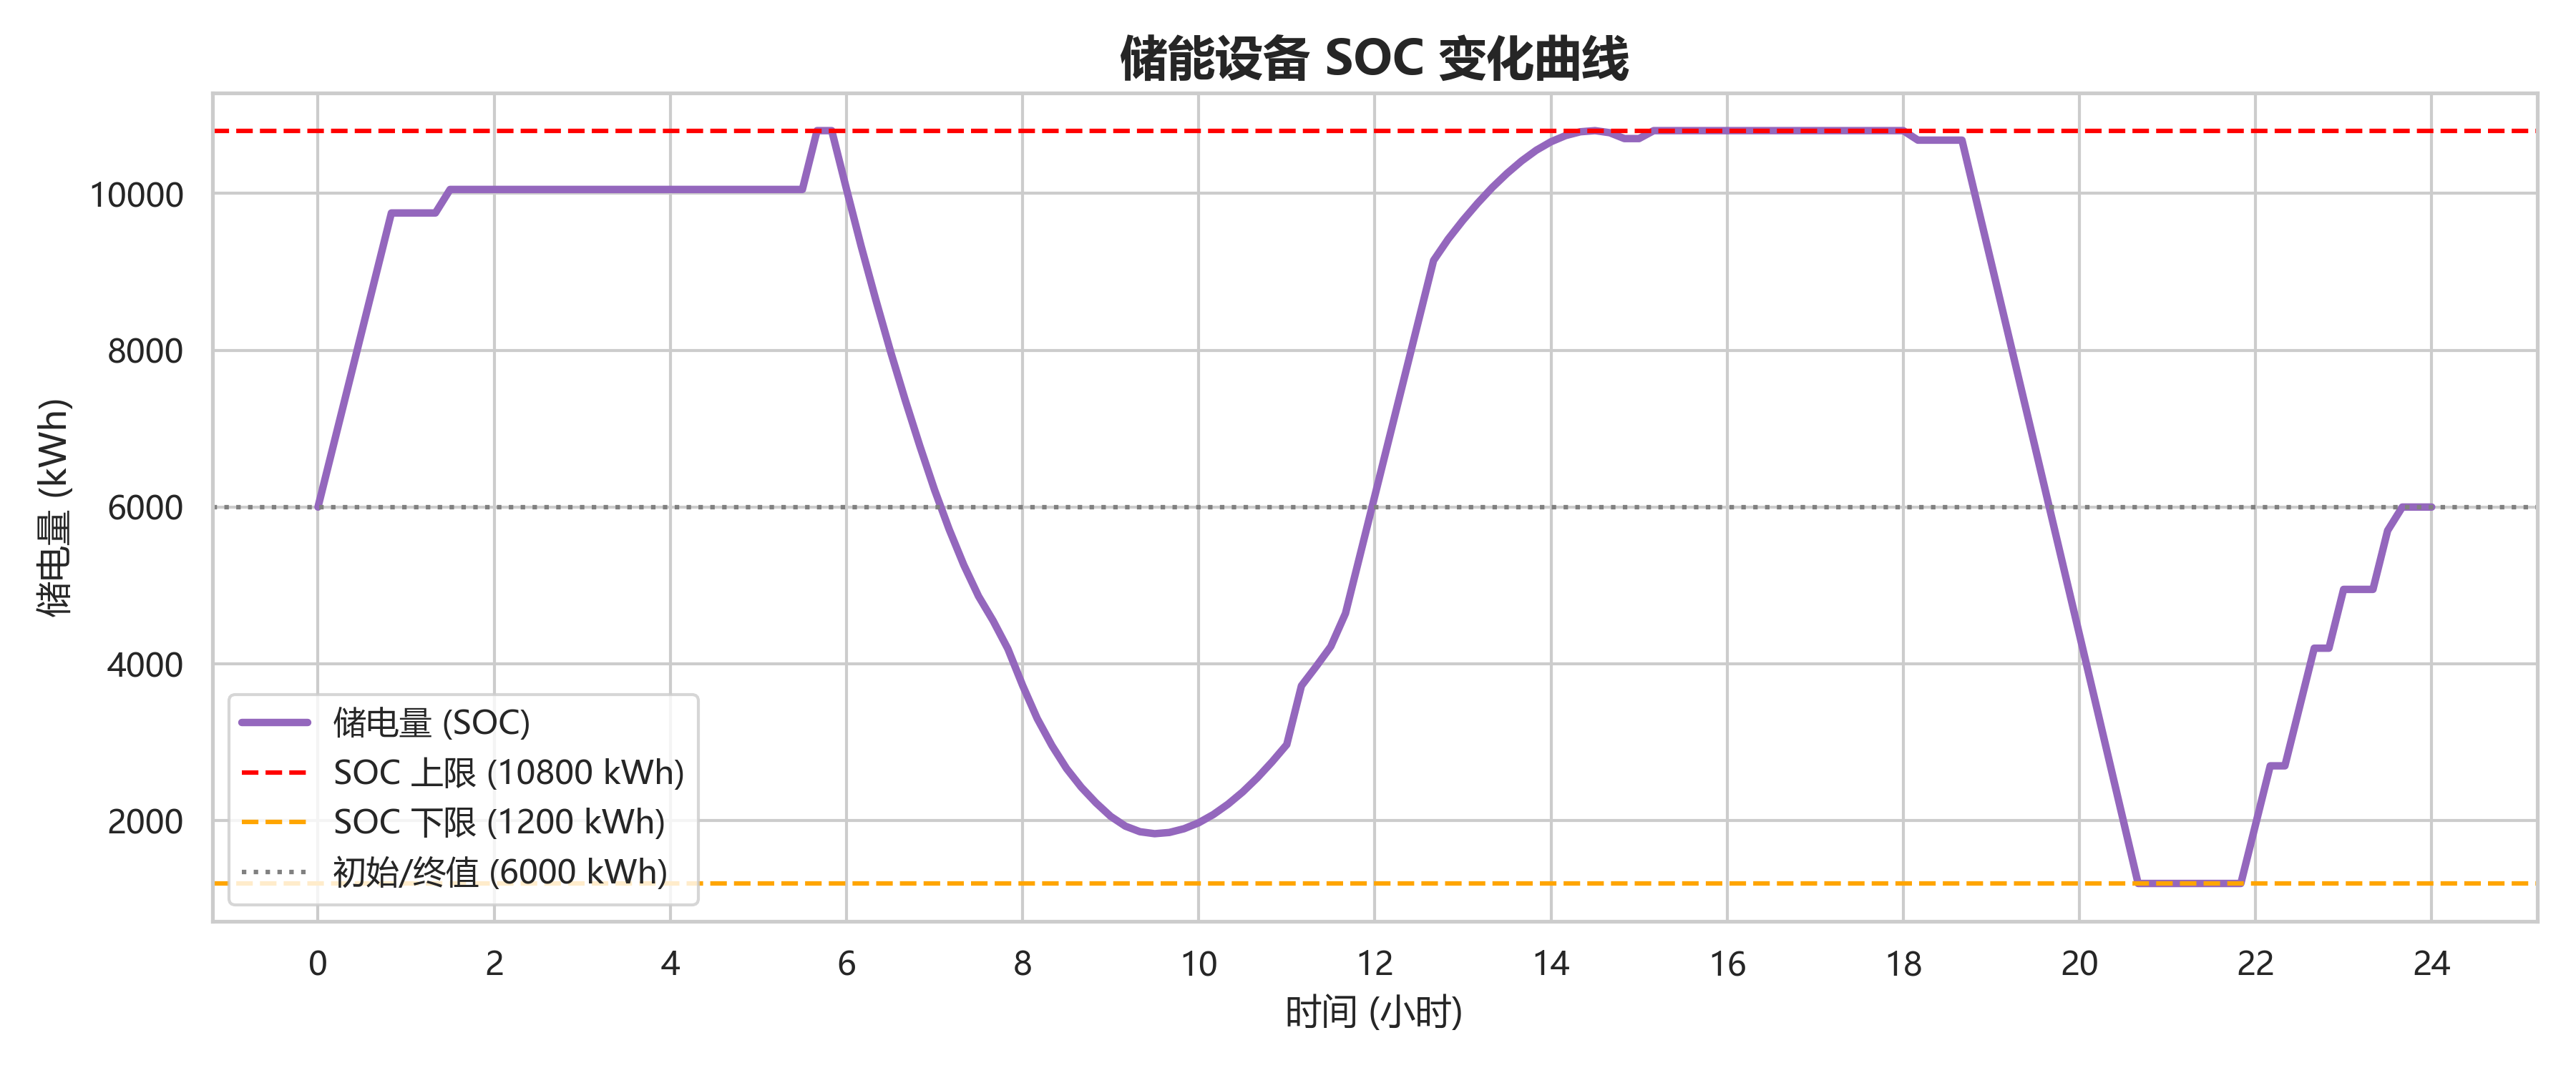
\includegraphics[width=.95\textwidth]{q1_soc.png}
\caption{问题一储能储电量变化}
\label{fig:q1soc}
\end{figure}

表~\ref{tab:q1dispatch4h}将十分钟结果汇总为题目要求的四小时区间。低价时段主要充电，16:00--20:00集中放电，调度轨迹与电价排序、光伏富余和日循环边界一致。

\begin{table}[H]
\centering
\normalsize
\setlength{\tabcolsep}{8pt}
\renewcommand\arraystretch{1.2}
\caption{问题一四小时储能调度汇总}
\label{tab:q1dispatch4h}
\begin{tabular}{lrrll}
\toprule
\textbf{时段} & \textbf{充电量（kWh）} & \textbf{放电量（kWh）} & \textbf{时刻} & \textbf{储电量（kWh）}\\
\midrule
0:00--4:00 & 4500.0000 & 0.0000 & 0:00 & 6000.0000\\
4:00--8:00 & 833.3333 & 6365.8412 & 24:00 & 6000.0000\\
8:00--12:00 & 4787.9643 & 1702.9970 & -- & --\\
12:00--16:00 & 5286.0352 & 91.1014 & -- & --\\
16:00--20:00 & 0.0000 & 5780.1319 & -- & --\\
20:00--24:00 & 5333.3333 & 2859.8681 & -- & --\\
\midrule
全天合计 & 20740.6661 & 16799.9396 & -- & --\\
\bottomrule
\end{tabular}
\end{table}

容量和效率敏感性实验显示，扩大容量或提高效率均可降低购电费用，但容量收益随规模扩大而递减；其原因是可利用的低价—高价价差和可转移电量有限。容量关系见图~\ref{fig:q1capacity}，完整扫描数据随支撑材料提交。

\begin{figure}[H]
\centering
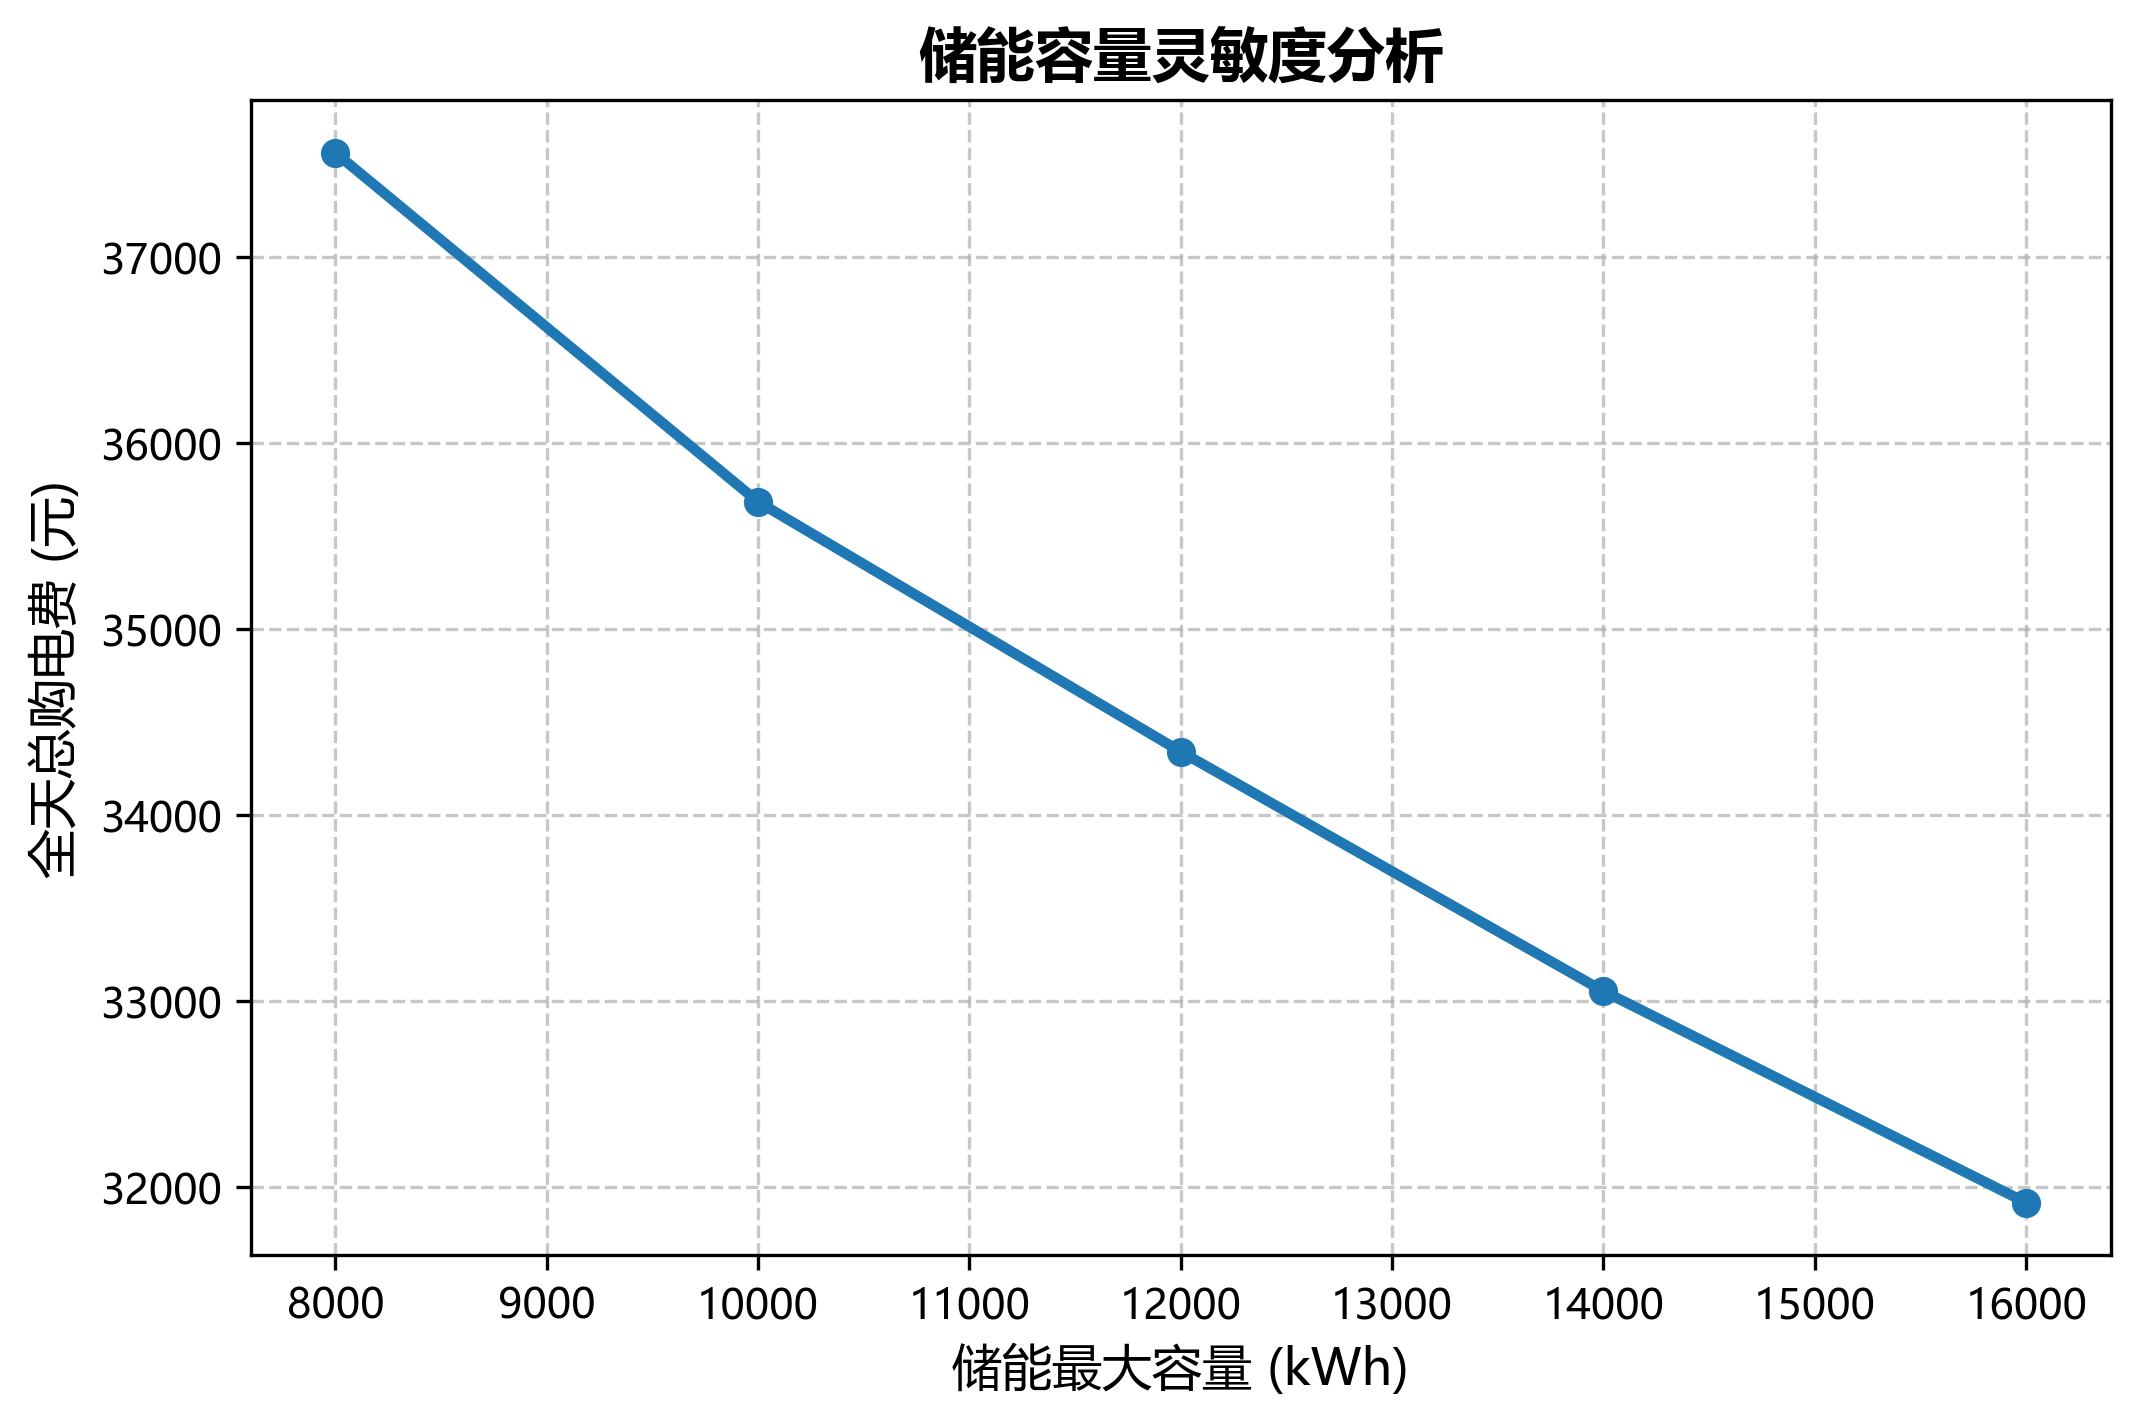
\includegraphics[width=.95\textwidth]{q1_capacity.png}
\caption{问题一储能容量敏感性}
\label{fig:q1capacity}
\end{figure}

微扰1 kWh负荷得到的影子价格为：02:00和12:00分别为0.4293和0.4411元/kWh，与外网电价一致；19:00为1.2561元/kWh，低于外网电价1.3523元/kWh，表明储能在该高价时段承担了部分边际需求。

\begin{table}[H]
\centering
\normalsize
\setlength{\tabcolsep}{8pt}
\renewcommand\arraystretch{1.2}
\caption{问题一典型时段边际供电成本}
\label{tab:q1shadow}
\begin{tabular}{lrrl}
\toprule
\textbf{时刻} & \textbf{外网电价} & \textbf{影子价格} & \textbf{解释}\\
\midrule
02:00 & 0.4293 & 0.4293 & 边际需求主要由外网满足\\
12:00 & 0.4411 & 0.4411 & 边际需求仍由外网补足\\
19:00 & 1.3523 & 1.2561 & 储能放电降低边际成本\\
\bottomrule
\end{tabular}
\end{table}

\subsection{问题二的模型建立与求解：机会约束日前优化与真实回测}

\subsubsection{具体分析}

问题二将问题一推广到全年历史回测，并限制每天0:00只能使用前14天历史净负荷。以$\mu_{d,t}+K\sigma_{d,t}$构造安全净负荷后，日前计划不再使用当天真实数据；真实负荷和光伏仅用于回测状态机。$K$过小会减少日前购电却增加紧急购电，$K$过大则相反。有限网格结果选定$K=0.80$，对应总成本1654.76万元、紧急购电量14.67万kWh；该选择是样本内的成本—风险折中，不代表全天联合可靠性。

\subsubsection{模型准备}

\paragraph{1. 数据预处理}

问题二在每天0:00制定全天计划，决策时不能使用当天真实负荷和光伏。对日期$d$，用前$W=14$天同一时段的净负荷样本计算
\begin{equation}
\mu_{d,t}=\frac{1}{W}\sum_{j=d-W}^{d-1}N_{j,t},\qquad
\sigma_{d,t}=\sqrt{\frac{1}{W}\sum_{j=d-W}^{d-1}(N_{j,t}-\mu_{d,t})^2}.
\tag{10}
\end{equation}
这里采用程序中的经验标准差（分母为$W$）；问题四4-2的程序则采用无偏标准差（分母为$W-1$），两者的计算口径分别保持与对应结果文件一致。

对日期$d$，$E^0_{d,t}$、$E_{\mathrm{ch},d,t}$、$E_{\mathrm{dis},d,t}$为日前决策变量，$S_{d,t}$为状态变量；$N_{d,t}$的当日真实值不属于0:00时的信息集，只在回测阶段使用。$\mu_{d,t}$和$\sigma_{d,t}$由历史窗口确定，$K$不进入内层线性规划的决策，而是由外层回测标定。

\paragraph{2. 算法选择}

在每天0:00信息集固定后，历史统计量可以将不确定的供电要求转化为确定的安全净负荷，因此日前决策仍可采用线性规划。考虑到当天真实数据只能在回测阶段使用，本文采用“机会约束日前规划+真实状态机回测”的两阶段算法：前一阶段生成不依赖当天真实数据的计划，后一阶段检验计划在真实负荷和实际光伏下的可执行性。该处理既保持机会约束模型的可解性，又避免使用未来信息造成结果偏乐观。

\subsubsection{模型建立}

在净负荷近似服从正态分布的条件下，对供电能力设置机会约束。机会约束的基本思想是允许小概率的约束违约，并通过分位点将概率要求转换为确定性安全裕度\cite{charnes1959,bental2009}：
\begin{equation}
\mathbb P\left(E^0_{d,t}+E_{\mathrm{dis},d,t}-E_{\mathrm{ch},d,t}\geq N_{d,t}\right)\geq1-\varepsilon
\tag{11}
\end{equation}
可转化为
\begin{equation}
E^0_{d,t}+E_{\mathrm{dis},d,t}-E_{\mathrm{ch},d,t}
\geq\mu_{d,t}+K\sigma_{d,t},\qquad K=\Phi^{-1}(1-\varepsilon).
\tag{12}
\end{equation}
这里的$K$是可调安全裕度系数。式（12）是逐时段确定性等价形式，不保证全天144个时段的联合覆盖率，因此需要结合全年回测选取$K$。

\subsubsection{模型求解}

对每个日期，算法依次执行“读取前14天历史数据—计算$\mu$和$\sigma$—给定$K$求解日前LP—代入真实负荷和光伏—按当前SOC执行储能补救—统计紧急购电、弃光和成本”。日期间不传递真实SOC，符合本文逐日闭环的评价口径。

日前线性规划目标为
\begin{equation}
\min Z_{2,\mathrm{DA}}=\sum_{t\in\Tset}p_tE^0_{d,t},
\tag{13}
\end{equation}
并结合式（4）至式（6）及式（12）。计划确定后，用当天真实数据计算实际净负荷缺口。日内不直接使用日前优化得到的充放电量，而是根据实际缺口和储能当前状态执行状态机：
\begin{equation}
\Delta E_{d,t}=E_{\mathrm{load},d,t}-E_{\mathrm{pv},d,t}-E^0_{d,t}.
\tag{14}
\end{equation}
\begin{equation}
E_{\mathrm{ch},d,t}^{\mathrm{real}}=
\begin{cases}
\min\left\{-\Delta E_{d,t},E_{\max},
\dfrac{S^{\max}-S_{d,t}^{\mathrm{real}}}{\eta_{\mathrm{ch}}}\right\},&\Delta E_{d,t}<0,\\
0,&\Delta E_{d,t}\geq0,
\end{cases}
\tag{14a}
\end{equation}
\begin{equation}
E_{\mathrm{dis},d,t}^{\mathrm{real}}=
\begin{cases}
\min\left\{\Delta E_{d,t},E_{\max},
\eta_{\mathrm{dis}}(S_{d,t}^{\mathrm{real}}-S^{\min})\right\},&\Delta E_{d,t}\geq0,\\
0,&\Delta E_{d,t}<0,
\end{cases}
\tag{14b}
\end{equation}
\begin{equation}
S_{d,t+1}^{\mathrm{real}}=S_{d,t}^{\mathrm{real}}+\eta_{\mathrm{ch}}E_{\mathrm{ch},d,t}^{\mathrm{real}}
-\frac{E_{\mathrm{dis},d,t}^{\mathrm{real}}}{\eta_{\mathrm{dis}}},\qquad S_{d,0}^{\mathrm{real}}=6000.
\tag{14c}
\end{equation}
放电后的剩余缺口和充电后的剩余富余分别记为
\begin{equation}
E_{\mathrm{emer},d,t}=\max\left\{0,\Delta E_{d,t}-E_{\mathrm{dis},d,t}^{\mathrm{real}}\right\},\qquad
E_{\mathrm{curt},d,t}=\max\left\{0,-\Delta E_{d,t}-E_{\mathrm{ch},d,t}^{\mathrm{real}}\right\}.
\tag{14d}
\end{equation}
式（6）的$S_{d,0}=S_{d,144}=6000$是日前计划的日循环约束；真实状态机只继承$S_{d,0}^{\mathrm{real}}=6000$，不再人为强制日末回到6000，因此指定日期的实际$24{:}00$储电量可能不同。该区分既保留了日前计划的可比性，也如实反映了真实数据冲击下的执行结果。
最终回测成本为
\begin{equation}
Z_2=\sum_{d,t}p_tE^0_{d,t}+5\sum_{d,t}p_tE_{\mathrm{emer},d,t}.
\tag{15}
\end{equation}
\paragraph{模型性质与执行逻辑}
式（13）的日前目标只计计划普通购电费；式（14）--（14d）把真实净负荷与计划之间的缺口交给储能状态机处理，储能受功率和SOC边界限制后的剩余缺口记为紧急购电，剩余富余记为弃光。这样，优化阶段与执行阶段的职责分离，且紧急购电不会被日前模型提前“看见”。

因此，日前计划和真实执行分别由预测数据与实际数据决定，避免了信息泄漏。

\paragraph{参数扫描与结果}

粗扫$K=0.40,0.50,\ldots,2.00$并在$0.80$--$0.85$区间细扫。总成本随$K$先降后升：$K=0.80$的总成本为1654.76万元，$K=0.81$仅低0.08万元，差异不足0.01\%，故选用更简洁的$K=0.80$；若优先考虑可靠性，可选$K=0.84$。

因此问题二采用“内层日前线性规划+外层样本内参数标定”的两层结构。令$\mathcal K$为候选安全系数集合，$Z_2(K)$为该系数在334天真实回测中的总成本，先求$Z_{\min}=\min_{K\in\mathcal K}Z_2(K)$，再在允许相对差异不超过$\delta=0.01\%$的候选中取最小$K$：
\begin{equation}
K_{\mathrm{main}}=\min\left\{K\in\mathcal K:Z_2(K)\leq(1+\delta)Z_{\min}\right\}.
\tag{15a}
\end{equation}
该规则将$K=0.80$的简洁性与$K=0.81$的微小成本差异纳入同一选择标准；若可靠性优先，则应报告相应风险指标并选取更大的$K$，而不能仅以总成本排序。

\begin{table}[H]
\centering
\normalsize
\setlength{\tabcolsep}{8pt}
\renewcommand\arraystretch{1.3}
\caption{问题二安全系数代表性扫描}
\label{tab:q2scan}
\begin{tabular}{ccrrr}
\toprule
$K$ & 总成本（万元） & 紧急天数 & 紧急购电（万kWh） & 弃光（万kWh）\\
\midrule
0.40 & 2058.18 & 233 & 112.87 & 380.15\\
0.60 & 1756.70 & 222 & 47.75 & 454.89\\
0.80 & \textbf{1654.76} & 122 & 14.67 & 560.70\\
0.81 & 1654.68 & 119 & 13.80 & 566.69\\
0.84 & 1656.62 & 105 & 11.52 & 584.99\\
1.00 & 1699.22 & 63 & 4.32 & 688.89\\
1.80 & 2128.62 & 1 & 0.00 & 1245.92\\
2.00 & 2245.78 & 0 & 0.00 & 1385.86\\
\bottomrule
\end{tabular}
\end{table}

固定$K=0.80$的回测中，日前购电费1564.61万元、紧急购电罚费90.15万元，合计1654.76万元；紧急购电发生于122天，共14.67万kWh，弃光560.70万kWh。动态安全裕度对照虽减少部分弃光，但增加了阴天欠购电和罚费，未作为主方案。

表~\ref{tab:q2datesummary}保留四个指定日期的核心回测指标；完整十分钟购电、四小时储能和紧急购电时段见附录结果文件。

\begin{table}[H]
\centering
\normalsize
\setlength{\tabcolsep}{8pt}
\renewcommand\arraystretch{1.3}
\caption{问题二指定日期核心回测指标}
\label{tab:q2datesummary}
\begin{tabular}{lrrrr}
\toprule
\textbf{日期} & \textbf{日前购电量} & \textbf{日前费用} & \textbf{紧急购电量} & \textbf{期末SOC}\\
& \multicolumn{1}{c}{(kWh)} & \multicolumn{1}{c}{(元)} & \multicolumn{1}{c}{(kWh)} & \multicolumn{1}{c}{(kWh)}\\
\midrule
2025-03-20 & 71619.93 & 43615.58 & 0.00 & 6482.54\\
2025-06-21 & 79970.15 & 49813.08 & 0.00 & 10800.00\\
2025-09-23 & 66442.78 & 41289.70 & 1116.51 & 6322.50\\
2025-12-21 & 96604.20 & 62017.16 & 0.00 & 6477.58\\
\bottomrule
\end{tabular}
\end{table}

表~\ref{tab:q2scan}显示，$K$从0.80增加到0.84可继续降低紧急购电，但总成本上升；$K=0.81$虽略低于主方案，仅改善0.08万元，故$K=0.80$仍作为经济性主方案。完整扫描数据见支撑材料。

四个指定日期中，仅2025-09-23出现紧急购电，合计1116.51 kWh；具体时段和逐时储能轨迹保留在附录结果文件中。

\subsection{问题三的模型建立与求解：光伏预测更新下的MPC滚动调度}

\subsubsection{具体分析}

问题三利用0:00、6:00、12:00和18:00更新的光伏预测，对未执行区间滚动重优化。预测经日期填充、跨日截断和十分钟插值后，再以$\beta$进行保守折减；每次更新只执行下一个区间，并以真实SOC作为下一次优化初值。$\beta=0.95$的MPC总成本为1368.87万元，较仅执行0:00计划节省8.03%，紧急购电量为14.3596万kWh。预测物理清洗可进一步降低风险，但增加常规购电，因此作为对照而非主方案。

\subsubsection{模型准备}

\paragraph{1. 数据预处理}

附件3在每天0:00、6:00、12:00和18:00给出未来24小时的整点光伏预测。读取后先对日期列向前填充，再按发布时间分组。6:00预报只取当天7:00至24:00，12:00预报只取当天13:00至24:00，18:00预报只取当天19:00至24:00，跨日部分不进入当天剩余时域。这里的截断是信息边界处理，而不是对跨日预测值进行重新计算。

为与十分钟决策变量对齐，程序以每个十分钟时段的中心时刻作为插值位置，即第$i$个切片对应$t_i=(i+1.5)/6$小时。0:00预测使用整点网格$0,1,\ldots,24$，在0点补入光伏功率0后进行线性插值；6:00、12:00和18:00预测分别以真实光伏序列在第35、71和107个零基切片处的功率作为当前时刻锚点，再连接当天剩余预测整点值并插值。这样既保持了当前运行状态与最新实测值的一致，也避免把次日预测误用于当日剩余时段。对插值后的日内预测乘以保守折减系数$\beta$：
\begin{equation}
\widetilde E_{\mathrm{pv},d,t}^{(r)}=\beta\widehat E_{\mathrm{pv},d,t}^{(r)},\qquad r\in\{6,12,18\}.
\tag{16}
\end{equation}
其中$\widehat E^{(0)}_{\mathrm{pv},d,t}$表示由附件3的0:00预报插值得到的全天光伏预测电量，$\widehat E^{(r)}_{\mathrm{pv},d,t}$表示发布时间$r$对应的剩余时段预测电量。主方案取$\beta=0.95$。$\beta$越小，预测越保守，通常会降低紧急购电，却可能增加常规购电和偏差成本。

0:00时的决策变量为全天计划购电量、充放电量和SOC；在更新时刻，已执行区间的变量固定，剩余区间的调整购电量、充放电量和SOC重新决策。已知输入包括截至当前时刻的真实SOC、已发布的光伏预测、负荷计划和基础电价；当天尚未发生区间的真实光伏只用于事后回测，不进入滚动优化。$\beta$是外层标定参数，不是内层LP变量。

\paragraph{2. 算法选择}

问题三的主要困难不是单次优化规模，而是预测信息在日内逐步到达。若每天只求解一次，已执行决策无法利用新预测修正；若直接使用全天真实数据，又会违反决策时的信息边界。因此选择模型预测控制（MPC）：在每个预报时刻以最新预测和当前真实储能状态重优化剩余时域，只执行下一个控制区间。由于购电、充放电和偏差辅助变量之间仍为线性关系，各滚动阶段均可调用线性规划求解器。

\subsubsection{模型建立}

0:00使用全天预测求解
\begin{equation}
\min Z_{3,0}=\sum_{t\in\Tset}p_tE^0_{d,t},qquad
E^0_{d,t}+E_{\mathrm{dis},d,t}-E_{\mathrm{ch},d,t}
\geq E_{\mathrm{load},d,t}-\widehat E^{(0)}_{\mathrm{pv},d,t}.
\tag{17}
\end{equation}
在更新断面$\tau\in\{35,71,107\}$，锁定已执行时段，以当前运行状态$S_{d,\tau}^{\mathrm{real}}$为初值，对剩余时域再优化。令$E_{d,t}$为调整后购电量，引入
\begin{equation}
E_{d,t}-E^0_{d,t}=u^+_{d,t}-u^-_{d,t},qquad u^+_{d,t},u^-_{d,t}\geq0.
\tag{18}
\end{equation}
根据题意，超计划购电按1.5倍电价，少购部分按原计划电价的50\%收取偏差费用。因此每一阶段的目标可写为
\begin{equation}
\min Z_{3,\tau}=\sum_{t=\tau}^{143}p_t
\left(E_{d,t}+0.5u^+_{d,t}+0.5u^-_{d,t}\right),
\tag{19}
\end{equation}
约束为
\begin{equation}
E_{d,t}+E_{\mathrm{dis},d,t}-E_{\mathrm{ch},d,t}
\geq E_{\mathrm{load},d,t}-\widetilde E_{\mathrm{pv},d,t}^{(\tau)}.
\tag{20}
\end{equation}
\paragraph{模型性质与约束含义}
式（18）中$u^+$和$u^-$分别表示增购和退订偏差。由于二者在目标函数中均产生正费用，最优解不会同时取正，从而在不增加二进制变量的情况下实现绝对偏差的线性化。式（20）保证最新预测下的供需覆盖，式（4）--（6）保证储能状态连续、功率和容量可行；已执行区间锁定后，下一阶段只能从当前真实SOC继续决策。
每次求解只执行下一个更新区间，全天购电和储能轨迹按模型预测控制的滚动时域思想拼接\cite{maciejowski2002,parisio2014}：
\begin{equation}
E^{\mathrm{exec}}=\left[E^0_{0:35},E^6_{35:71},E^{12}_{71:107},E^{18}_{107:144}\right]
\tag{21}
\end{equation}
拼接。真实回测使用附件2的实际负荷和实际光伏，紧急购电量为
\begin{equation}
E_{\mathrm{emer},d,t}=\max\left\{0,E_{\mathrm{load},d,t}-E_{\mathrm{pv},d,t}
-E^{\mathrm{exec}}_{d,t}-E^{\mathrm{exec}}_{\mathrm{dis},d,t}
+E^{\mathrm{exec}}_{\mathrm{ch},d,t}\right\}.
\tag{22}
\end{equation}

问题三原文只明确给出计划偏差结算规则，本文沿用问题二的紧急购电按交易时刻电价5倍的口径。日总成本为常规购电、偏差费用和紧急购电费用之和：
\begin{equation}
C_{3,d}=\sum_t p_tE^{\mathrm{exec}}_{d,t}
+0.5\sum_t p_t|E^{\mathrm{exec}}_{d,t}-E^0_{d,t}|
+5\sum_t p_tE_{\mathrm{emer},d,t}.
\tag{23}
\end{equation}

\subsubsection{模型求解}

问题三的执行流程为“0:00生成全天计划—执行0:00--6:00区间—读取6:00真实SOC和新预报—重优化6:00--12:00区间—依次完成12:00和18:00更新—拼接四段已执行轨迹—代入真实负荷和实际光伏结算”。该流程保证后续预测只影响未执行区间。

\begin{table}[H]
\centering
\renewcommand\arraystretch{1.2}
\caption{问题三滚动策略回测对比}
\label{tab:q3result}
\begin{tabular}{lrrr}
\toprule
\textbf{策略} & 总成本（万元） & 紧急购电（万kWh） & 节省比例\\
\midrule
仅执行0:00计划 & 1488.33 & 62.3295 & --\\
MPC，$\beta=1.00$ & 1403.07 & 34.6951 & 5.73\%\\
MPC，$\beta=0.98$ & 1376.30 & 23.7359 & 7.53\%\\
MPC，$\beta=0.95$ & \textbf{1368.87} & 14.3596 & \textbf{8.03\%}\\
MPC，$\beta=0.90$ & 1409.64 & 8.9414 & 5.29\%\\
\bottomrule
\end{tabular}
\end{table}

主方案的成本由实际购电1275.68万元、偏差费用35.90万元和紧急购电费用57.29万元构成。与静态0:00计划相比，MPC同时降低综合成本和紧急购电量；$\beta$继续降低虽可减少风险，但会增加常规购电和偏差费用。四个发布时间的光伏预测平均绝对误差依次为207.47、176.44、88.79和7.20 kW，6:00误差与当日紧急购电量的Pearson相关系数为0.660；该相关性仅用于风险解释，不作因果结论。

\paragraph{保守折减系数的敏感性}

保持数据、滚动时点、储能边界和费用口径不变，仅改变$\beta$。$\beta$从1.00降至0.95时，紧急购电量由34.6951万kWh降至14.3596万kWh且总成本下降；继续降至0.90后，风险继续下降但常规购电和偏差费用上升，总成本回升。因此，$\beta=0.95$是本样本候选网格中的经济性折中点。

令$\mathcal B$为候选折减系数集合，$Z_3(\beta)$为对应334天回测总成本，则内层滚动LP与外层参数标定可写为
\begin{equation}
\beta^*=\arg\min_{\beta\in\mathcal B} Z_3(\beta),
\tag{23a}
\end{equation}
本实验网格上$\beta^*=0.95$；若运行目标改为优先降低紧急购电量，则应改用风险约束或多目标选择，而不能继续使用单纯成本最小准则。

图~\ref{fig:q3sensitivity}保留成本—风险权衡的趋势，完整数据见支撑材料。

\begin{figure}[H]
\centering
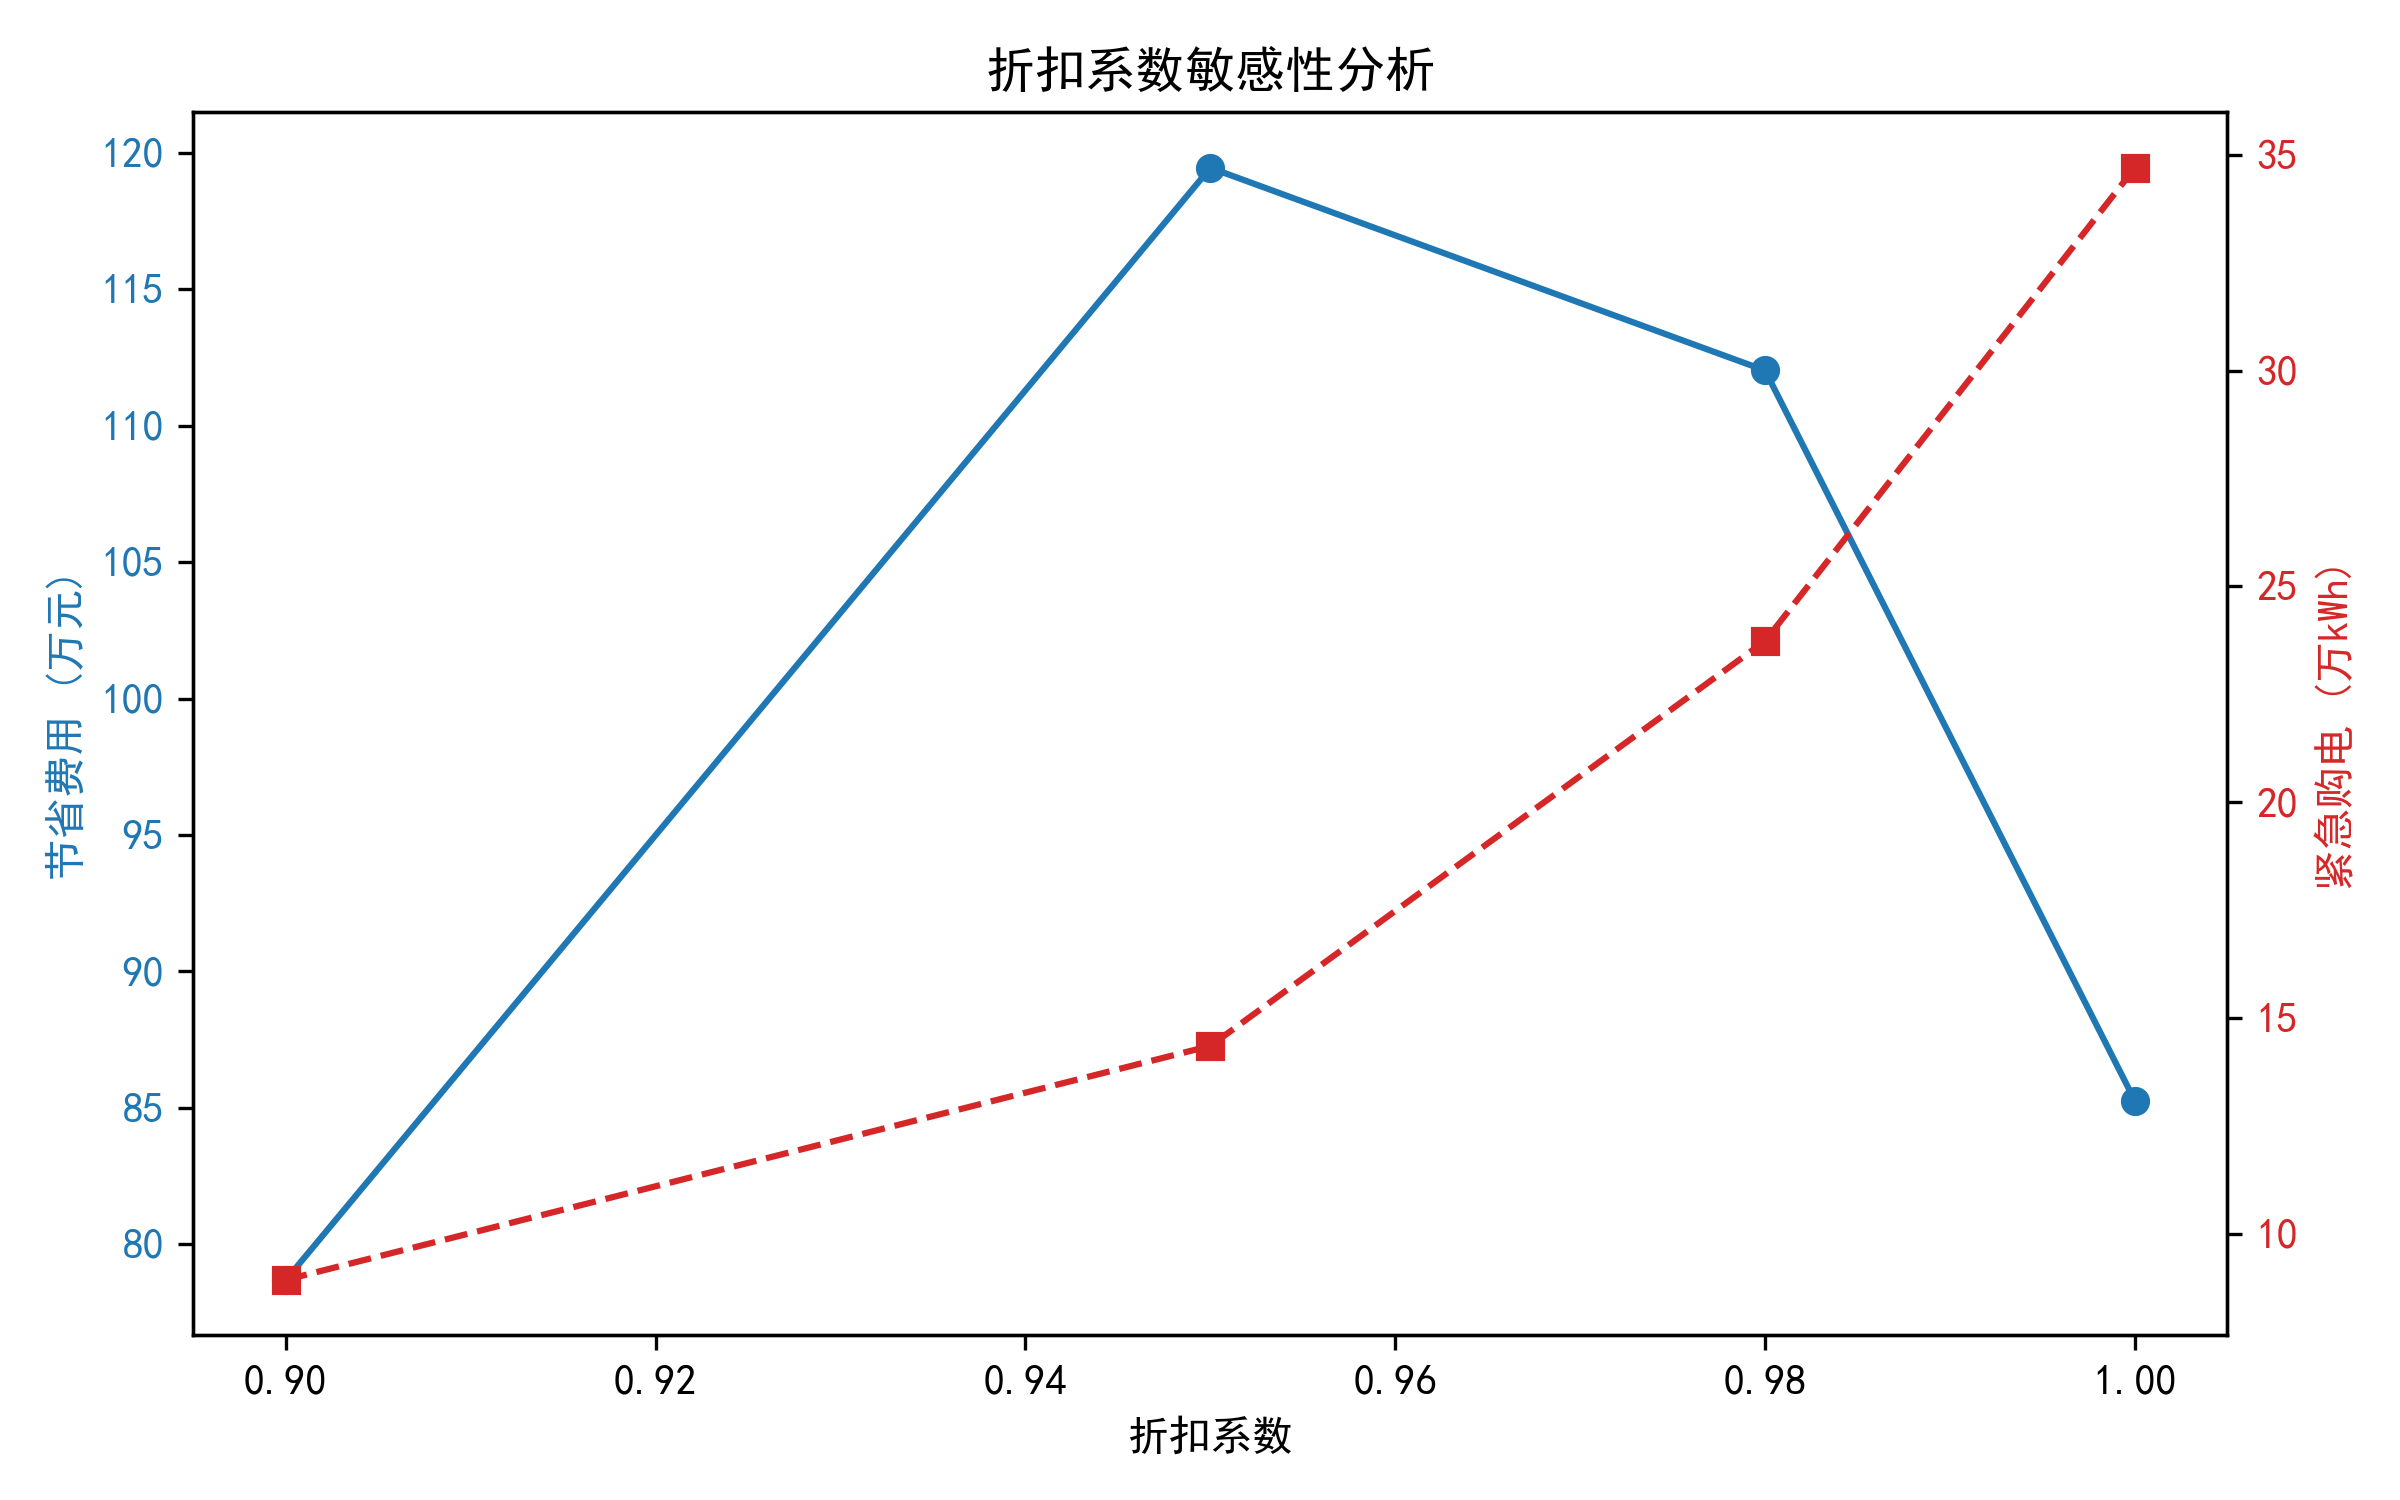
\includegraphics[width=.80\textwidth]{q3_sensitivity.png}
\caption{问题三预测折减系数敏感性曲线}
\label{fig:q3sensitivity}
\end{figure}

\paragraph{其他预报时刻的必要性分析}

在334天样本上，预测MAE由0:00的207.47 kW降至18:00的7.20 kW，新增信息的误差修正空间随发布时间缩小；同时，本文未对更高频更新进行独立对照，因此只能认为现有四个断面在本数据和费用口径下足以支撑主方案，不能推出普遍最优性。

\paragraph{成本构成与典型日期核验}

主方案的实际购电、偏差和紧急购电费用分别占总成本的93.19\%、2.62\%和4.19\%，主要收益来自购电与储能时序的改善；光伏快速变化或储能功率受限时仍会产生紧急购电。

表~\ref{tab:q3dates}给出四个季节代表日的核心回测指标；完整十分钟购电、滚动储能动作和紧急购电时段见附录结果文件。

\begin{table}[H]
\centering
\normalsize
\setlength{\tabcolsep}{8pt}
\renewcommand\arraystretch{1.3}
\caption{问题三指定日期核心回测指标}
\label{tab:q3dates}
\begin{tabular}{lrrrr}
\toprule
\textbf{日期} & \textbf{调整购电量} & \textbf{总费用} & \textbf{紧急购电量} & \textbf{期末SOC}\\
& \multicolumn{1}{c}{(kWh)} & \multicolumn{1}{c}{(元)} & \multicolumn{1}{c}{(kWh)} & \multicolumn{1}{c}{(kWh)}\\
\midrule
2025-03-20 & 66910.26 & 45359.49 & 1063.55 & 6000.00\\
2025-06-21 & 33732.47 & 19530.85 & 192.14 & 6000.00\\
2025-09-23 & 69276.70 & 44903.98 & 275.37 & 6000.00\\
2025-12-21 & 95483.20 & 63356.73 & 512.22 & 6000.00\\
\bottomrule
\end{tabular}
\end{table}

紧急购电主要集中于清晨光伏爬坡阶段；不同季节的发生区间随日出时间和爬坡速度变化。完整轨迹随支撑材料提交。

\paragraph{改进方案的消融实验}

为判断风险是否主要来自光伏预报的物理不合理片段，方案A将日出前、日落后的预测置零，并将6:30--8:30的晨间爬坡预测乘以0.75。在$\beta=0.95$下，方案A把紧急购电量从14.3596万kWh降至4.7014万kWh，但总成本由1368.87万元升至1379.37万元。进一步在方案A上把5:00--8:00的储能最低电量由1200提高到2000 kWh，得到方案A+B总成本1381.24万元，紧急购电量仍为4.7014万kWh。

物理清洗将紧急购电量降至4.7014万kWh，但总成本升至1379.37万元；叠加晨间SOC下限后成本进一步升至1381.24万元且风险未继续下降。图~\ref{fig:q3cleancompare}表明，当前改进的主要代价是增加常规购电，限制因素更可能是预测误差和放电功率。

\begin{figure}[H]
\centering
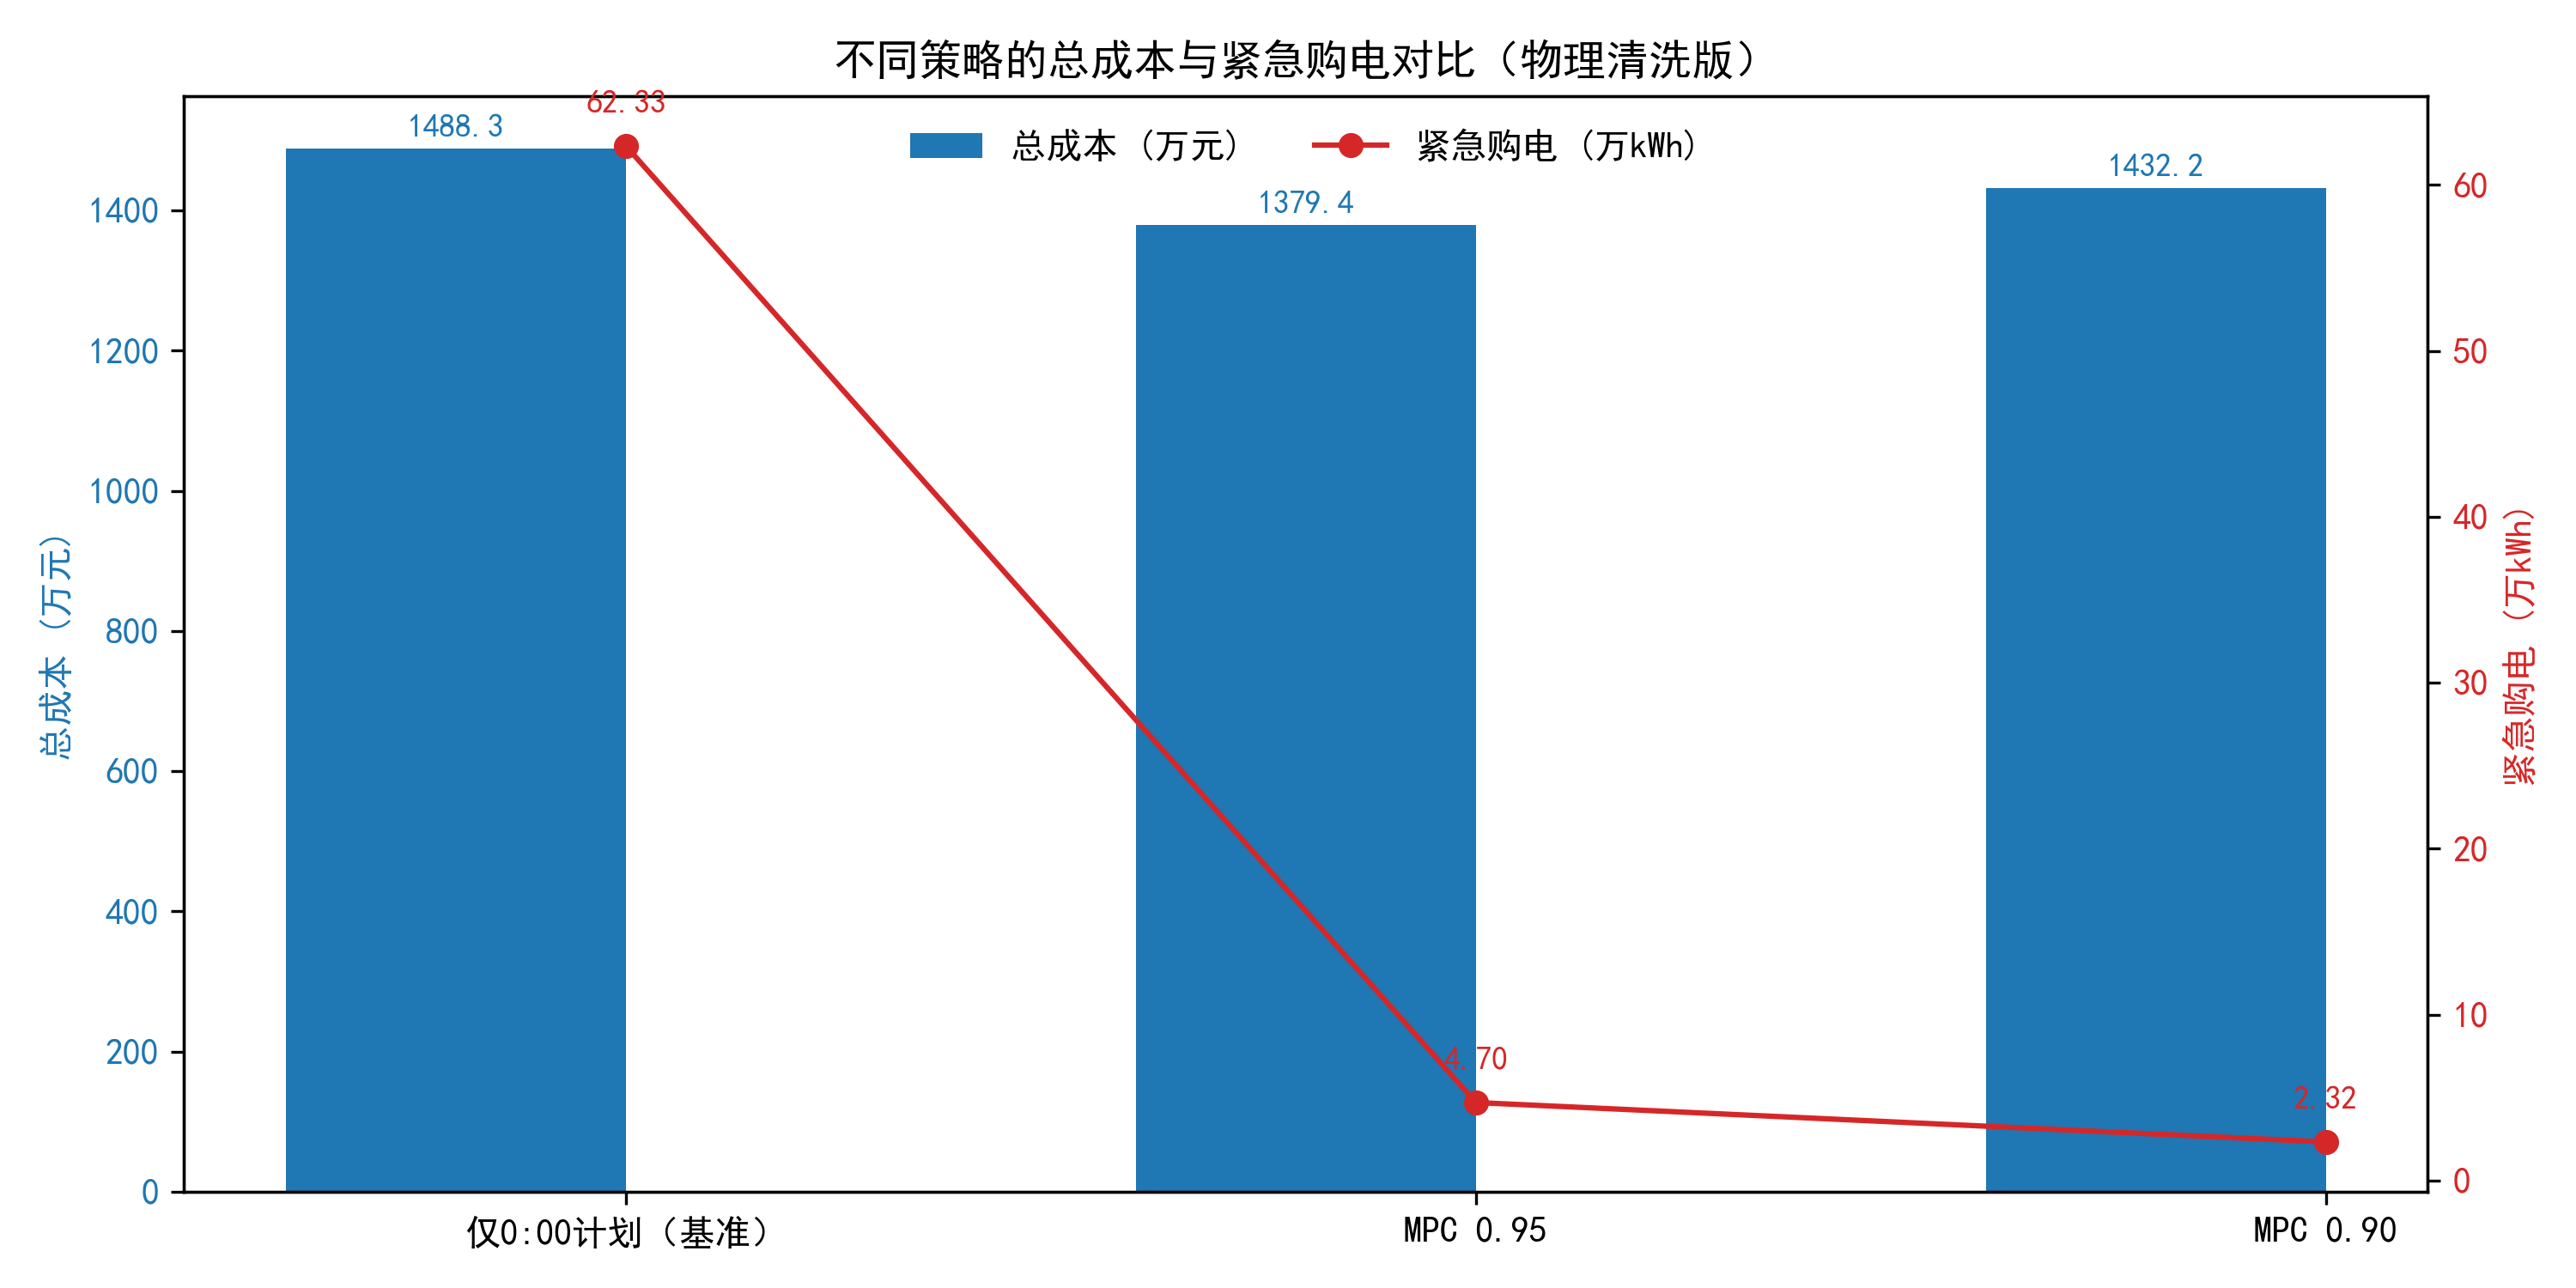
\includegraphics[width=.95\textwidth]{q3_clean_compare.png}
\caption{问题三预测清洗与SOC下限的消融实验}
\label{fig:q3cleancompare}
\end{figure}

\subsection{问题四的模型建立与求解：动态电价下的机会约束与MPC}

\subsubsection{具体分析}

问题四在问题二、三的信息结构上引入日期—时段动态电价。4-2用于评价动态价格下的机会约束日前调度，4-3用于评价动态价格下的MPC调度。4-2与4-3的跨模型差异不能单独归因于滚动机制，因此另设相同4-3信息和价格下的0:00固定计划基准。回测中4-2和4-3总成本分别为1740.24万元和1433.19万元；同一4-3模型中，MPC较固定计划节省121.14万元，节省率7.79%。

\subsubsection{模型准备}

\paragraph{1. 数据预处理}

问题四在问题二、问题三的数据处理基础上，引入附件4按日期和十分钟时段给出的动态电价矩阵$C_{d,t}$。程序将动态电价与负荷、实际光伏和预测光伏按日期及十分钟索引对齐，并保持问题二至问题三的电量单位、储能边界、334天回测区间和日循环边界不变。这样，问题四的成本变化可以归因于价格输入和决策机制，而不是数据维度或设备参数变化。

4-2的外层输入为前14天历史净负荷统计量和当日动态电价，内层决策变量为日前购电、充放电及SOC；4-3进一步使用四次预报和当前真实SOC，决策变量为滚动调整购电、充放电及偏差辅助变量。$K$和$\beta$均为外层参数：$K$改变日前安全净负荷，$\beta$改变日内光伏预测，二者不直接作为LP变量。

\paragraph{2. 算法选择}

问题四同时包含不确定光伏、动态价格和日内信息更新。4-2沿用机会约束日前规划，检验动态价格对安全裕度选择和储能套利的影响；4-3沿用MPC滚动规划，检验在相同动态价格下预测更新的边际价值。两类模型的约束结构仍为线性，故统一采用线性规划求解，并通过“4-2与4-3跨模型比较”和“4-3固定计划与MPC同模型比较”区分不同机制的作用。

\subsubsection{模型建立}

问题四将基础价格替换为附件4的动态电价矩阵$C_{d,t}$。对4-2，使用式（10）的历史统计量和安全净负荷$\mu_{d,t}+K\sigma_{d,t}$，目标函数为
\begin{equation}
\min Z_{4-2,\mathrm{DA}}=\sum_{t\in\Tset}C_{d,t}E^0_{d,t}.
\tag{24}
\end{equation}
实际结算仍按
\begin{equation}
Z_{4-2}=\sum_{d,t}C_{d,t}E^0_{d,t}+5\sum_{d,t}C_{d,t}E_{\mathrm{emer},d,t}.
\tag{25}
\end{equation}

对4-3，MPC的预测供需平衡使用动态电价下的调整购电量：
\begin{equation}
E_{d,t}+\widetilde E_{\mathrm{pv},d,t}^{(\tau)}+E_{\mathrm{dis},d,t}-E_{\mathrm{ch},d,t}
\geq E_{\mathrm{load},d,t},qquad t\geq\tau,
\tag{26}
\end{equation}
其偏差费用线性化目标为
\begin{equation}
\min Z_{4-3,\tau}=\sum_{t=\tau}^{143}C_{d,t}
\left(E_{d,t}+0.5u^+_{d,t}+0.5u^-_{d,t}\right).
\tag{27}
\end{equation}
\paragraph{模型性质与结算逻辑}
式（24）和式（27）分别最小化动态价格下的日前购电成本和滚动结算成本；式（25）将真实缺口按5倍动态电价结算。式（26）保证预测供需覆盖，式（28）--（30）保证实际执行轨迹满足能量守恒，并分别识别紧急购电与弃光。固定$K$或$\beta$后，历史统计量和价格均为已知参数，模型仍是连续线性规划；偏差变量的正成本使$u^+$与$u^-$不会同时为正。

真实回测使用附件2的负荷和实际光伏；主场景取$K=0.80$、$\beta=0.95$，紧急购电按5倍动态电价结算。4-2的储能动作为日前计划，4-3的动作为各滚动阶段锁定的执行轨迹，已执行区间不因后续信息反向修改。记最终执行轨迹为$E_{\mathrm{ch},d,t}^{\mathrm{exec}}$和$E_{\mathrm{dis},d,t}^{\mathrm{exec}}$，则
\begin{equation}
S_{d,t+1}^{\mathrm{exec}}=S_{d,t}^{\mathrm{exec}}+0.9E_{\mathrm{ch},d,t}^{\mathrm{exec}}
-\frac{E_{\mathrm{dis},d,t}^{\mathrm{exec}}}{0.9},\qquad S_{d,0}^{\mathrm{exec}}=6000,
\tag{28}
\end{equation}
并以$E_{\mathrm{buy},d,t}$表示4-2的日前购电量或4-3的最终调整购电量，计算
\begin{equation}
R_{d,t}=E_{\mathrm{pv},d,t}+E_{\mathrm{buy},d,t}+E_{\mathrm{dis},d,t}^{\mathrm{exec}}
-E_{\mathrm{ch},d,t}^{\mathrm{exec}}-E_{\mathrm{load},d,t},
\tag{29}
\end{equation}
\begin{equation}
E_{\mathrm{emer},d,t}=\max\{0,-R_{d,t}\},\qquad
E_{\mathrm{curt},d,t}=\max\{0,R_{d,t}\}.
\tag{30}
\end{equation}
式（28）--（30）明确了实际数据进入状态递推和缺口结算的路径。

\subsubsection{模型求解}

4-2的流程为“历史统计—构造安全净负荷—输入动态电价—求解日前LP—代入真实数据回测”；4-3的流程为“0:00生成初始计划—按6:00、12:00、18:00更新预测—锁定已执行区间—继承真实SOC—重优化剩余区间—按动态电价结算”。两类模型均输出成本、紧急购电、弃光和SOC校验结果。

\begin{table}[H]
\centering
\renewcommand\arraystretch{1.2}
\caption{动态电价方案回测对比}
\label{tab:q4main}
\begin{tabular}{lrr}
\toprule
\textbf{指标} & \textbf{4-2} & \textbf{4-3 MPC}\\
\midrule
回测天数 & 334 & 334\\
总成本（万元） & 1740.2419 & \textbf{1433.1927}\\
普通购电或结算成本（万元） & 1578.6095 & 1374.2854\\
紧急购电成本（万元） & 161.6324 & 58.9073\\
紧急购电量（万kWh） & 37.0508 & 14.3723\\
紧急购电天数 & 246 & 334\\
弃光量（万kWh） & 625.1011 & 188.4382\\
\bottomrule
\end{tabular}
\end{table}

4-3相较4-2将紧急购电量降至38.79\%、紧急购电成本降至36.45\%，弃光量下降69.86\%；但紧急购电天数由246天增至334天，说明风险总量下降并不等于发生天数下降。与同一4-3模型的0:00固定计划相比，MPC节省121.14万元，7.79\%的节省率可用于识别滚动机制的边际收益。

\paragraph{动态电价和参数敏感性}

附件4中价差最大的样本日为2025年8月15日。$K$扫描中$K=0.80$取得4-2最低总成本，$K=0.84$风险更低但成本略高；$\beta$扫描中$\beta=0.95$取得4-3最低总成本，$\beta=0.90$进一步降低紧急购电但成本回升。关键结果见表~\ref{tab:q4sens}，完整数据随支撑材料提交。

令$\mathcal K$和$\mathcal B$分别为候选参数集合，$Z_{4-2}(K)$和$Z_{4-3}(\beta)$为334天回测总成本，则参数选择可表示为
\begin{equation}
K^*=\arg\min_{K\in\mathcal K}Z_{4-2}(K),\qquad
\beta^*=\arg\min_{\beta\in\mathcal B}Z_{4-3}(\beta).
\tag{27a}
\end{equation}
实际主方案取$K=0.80$、$\beta=0.95$；两者分别来自对应候选网格的经济性折中选择，若改变风险偏好，应同时报告成本和紧急购电指标。

\begin{table}[H]
\centering
\renewcommand\arraystretch{1.2}
\caption{问题四关键参数敏感性摘要}
\label{tab:q4sens}
\begin{tabular}{ccrrr}
\toprule
\textbf{模型} & \textbf{参数} & 总成本（万元） & 紧急购电量（万kWh） & 备注\\
\midrule
4-2 & $K=0.70$ & 1757.7321 & 53.1217 & 风险较高\\
4-2 & $K=0.80$ & \textbf{1740.2419} & 37.0508 & 经济性主方案\\
4-2 & $K=0.90$ & 1746.8967 & 26.0479 & 可靠性优先\\
4-3 & $\beta=1.00$ & 1467.3062 & 34.7520 & 预测不折减\\
4-3 & $\beta=0.95$ & \textbf{1433.1927} & 14.3723 & 主方案\\
4-3 & $\beta=0.90$ & 1476.3934 & 8.9465 & 过度保守\\
\bottomrule
\end{tabular}
\end{table}

\paragraph{紧急购电与弃光的时段特征}

4-2的较高弃光量与日前安全裕度占用购电和储能空间有关；4-3利用新预测减少了不必要的购电和充电，因而弃光量下降。该解释是对334天样本的统计归纳，不外推至其他误差分布。

\paragraph{极端价差日的运行机理}

2025-08-15为回测期内价差最大日。图~\ref{fig:q4arbitrage}显示，SOC在低价时段上升、高价时段下降；该套利轨迹由动态价格进入目标函数后的最优解产生，相关数据见支撑材料。

\begin{figure}[H]
\centering
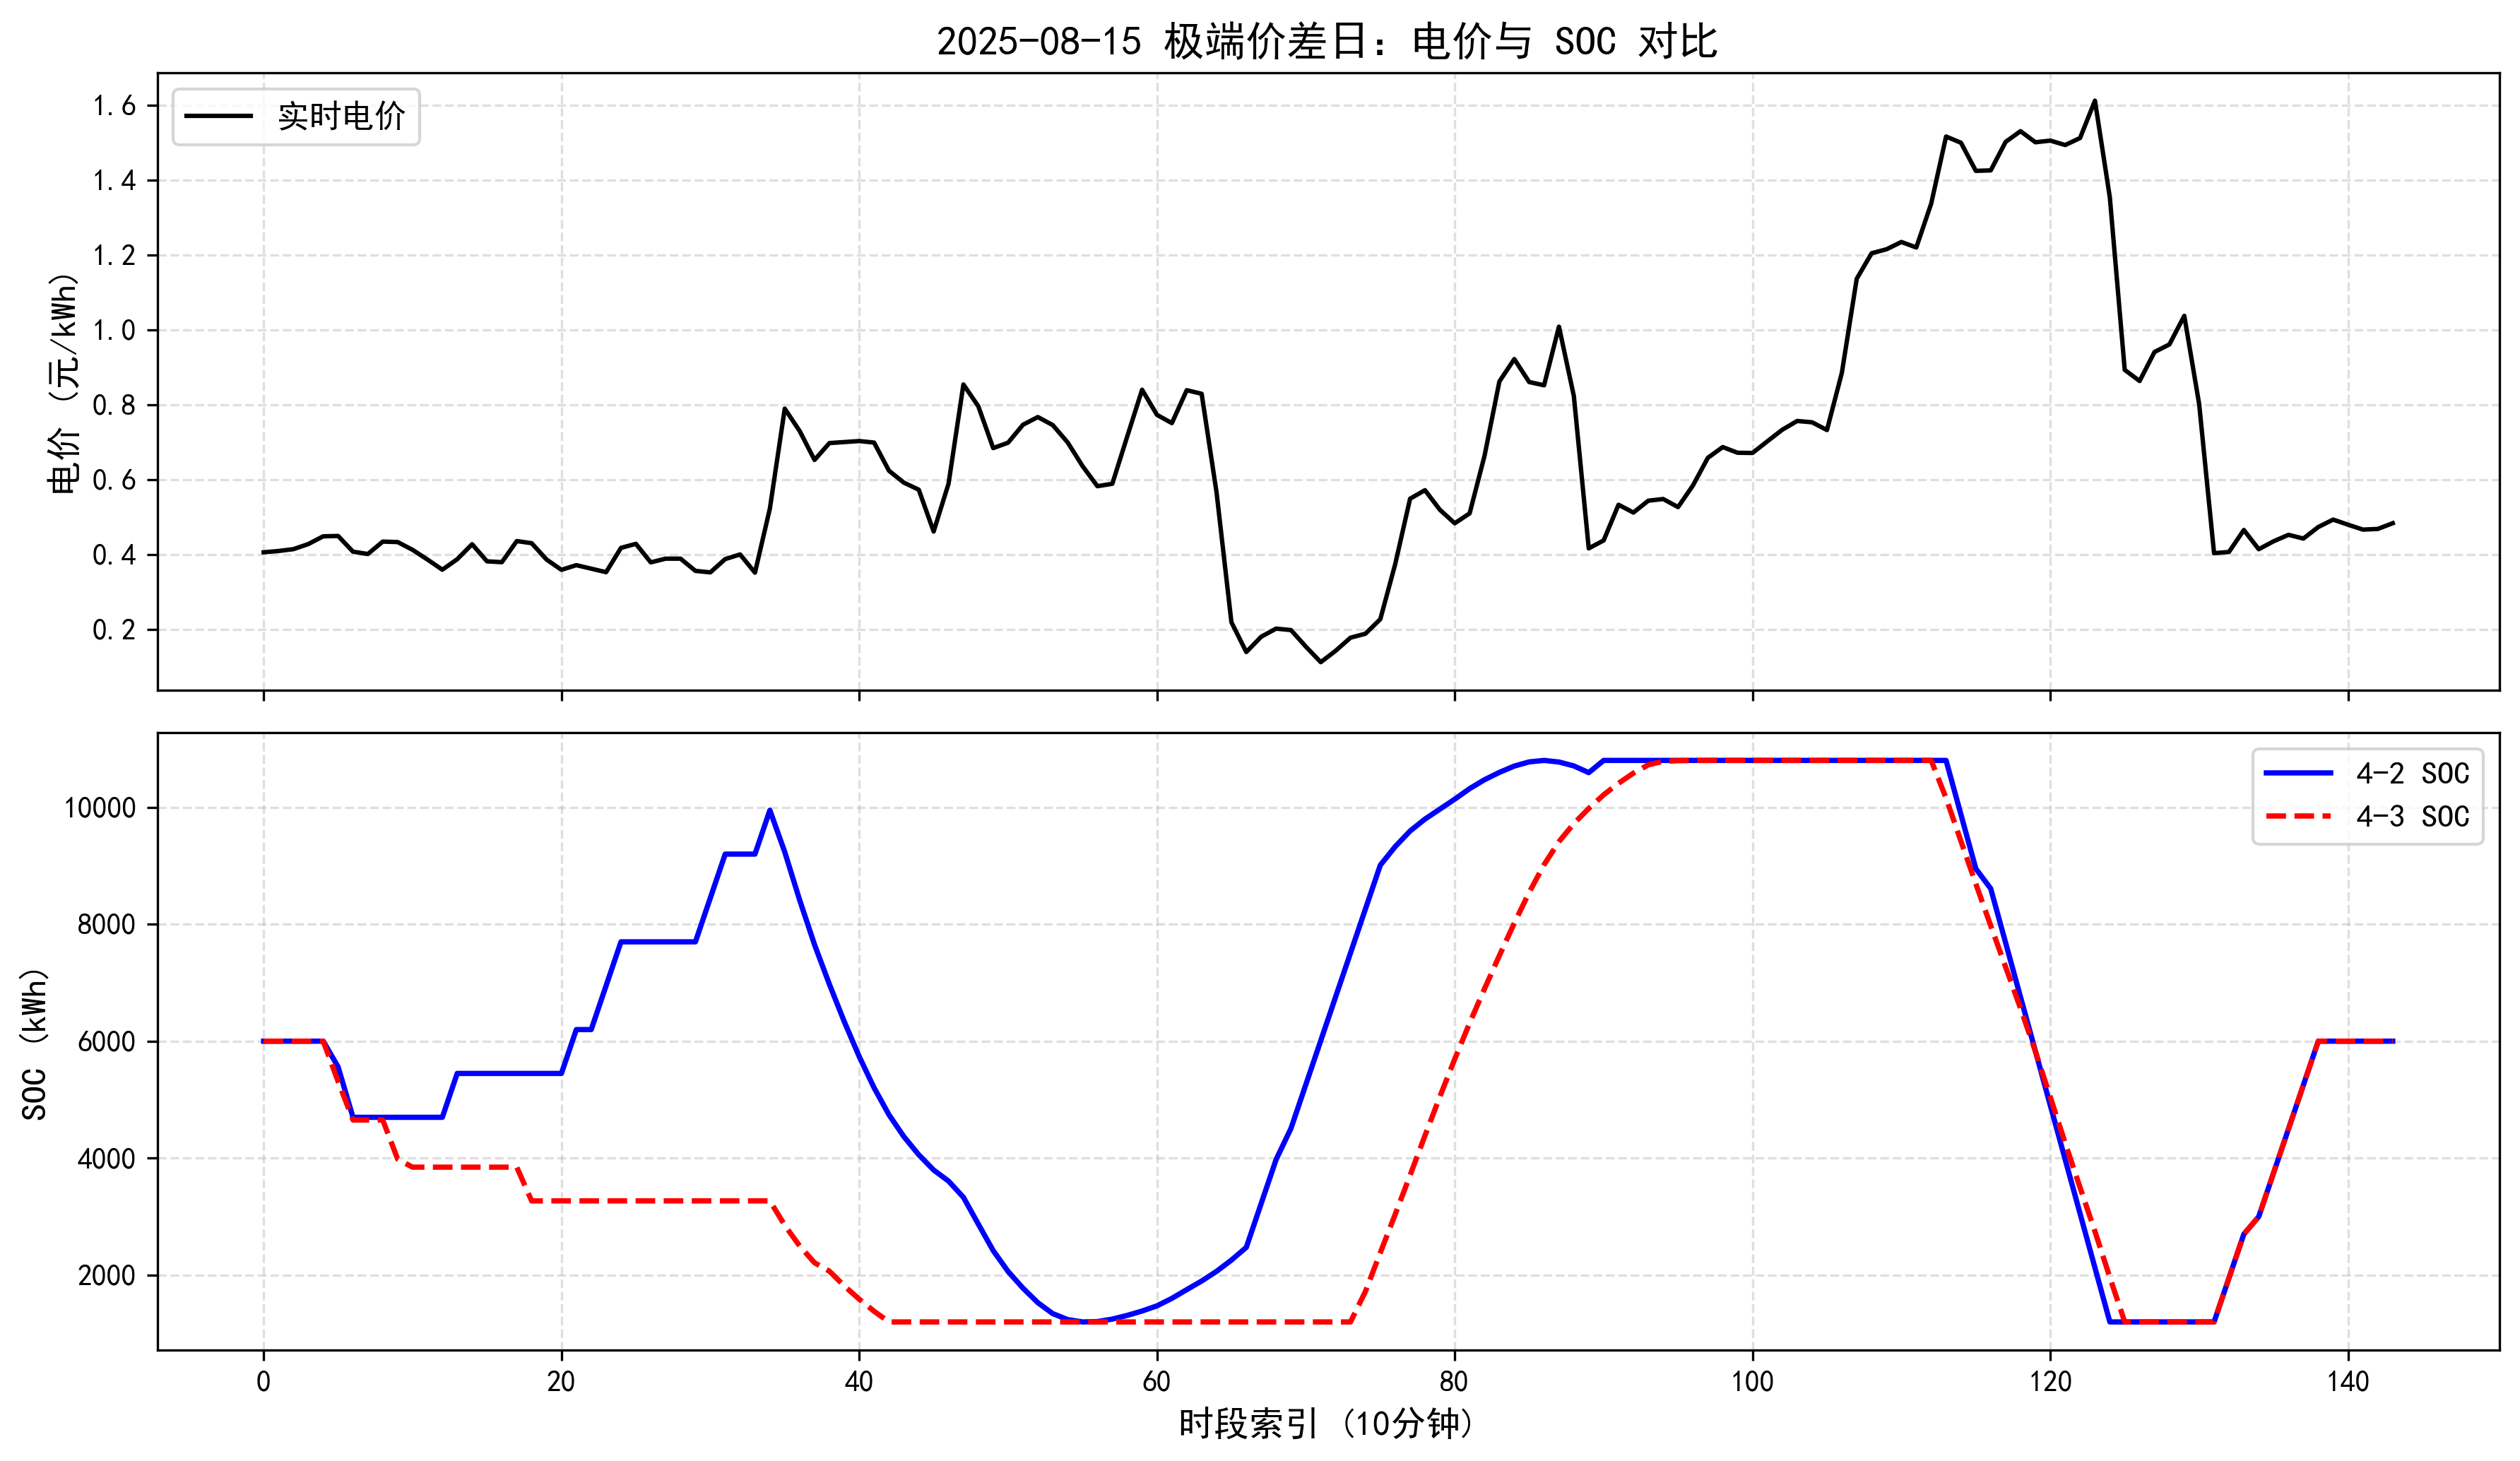
\includegraphics[width=.95\textwidth]{q4_arbitrage_soc.png}
\caption{2025-08-15动态电价与储能SOC}
\label{fig:q4arbitrage}
\end{figure}

参数实验均采用单因素变化，其余条件保持不变；由于参数在同一334天样本上选择，结果属于样本内比较，不能替代跨年份验证。

\section{模型检验与分析}

\subsection{模型精度验证}

四问均先将数据整理为按日期索引的144维十分钟电量序列，再在对应信息集下调用HiGHS求解线性规划。问题二和4-2使用前14天统计量，问题三和4-3对四次光伏预报进行插值和折减，并在更新时刻仅重优化未执行区间；回测阶段依据真实负荷、实际光伏和储能状态递推结算。该求解器给出的是给定预测、状态和费用规则下的单阶段最优，不等同于未知真实数据下的全局最优\cite{huangfu2018}。

\subsection{灵敏度分析}

敏感性分析仅改变一个参数，其余条件保持不变。结果具有一致的风险—成本规律：容量或效率提高的收益递减，$K$过小增加紧急购电，$K$过大增加日前购电和弃光，$\beta$存在成本较低的中间区间。因此，$K=0.80$和$\beta=0.95$均是给定样本、费用口径和参数网格下的选择，不构成普适最优性结论；完整扫描数据见支撑材料。

\subsection{结果合理性检验}

结果合理性检查包括四项：日期与144个时段完整匹配；线性规划均成功求解；SOC递推满足式（4）--（6）的边界和守恒；紧急购电与弃光由真实数据下的供需缺口计算，而非由优化器直接安排。四问的结果文件分别保存十分钟购电量、四小时储能汇总、始末SOC和紧急购电时段，核心代码与中间数据见附录和支撑材料。


\begin{table}[H]
\centering
\normalsize
\setlength{\tabcolsep}{8pt}
\renewcommand\arraystretch{1.25}
\caption{问题主要实验结论汇总}
\label{tab:overallresult}
\begin{tabular}{p{1.0cm}p{2.8cm}p{4.1cm}p{4.1cm}}
\toprule
\textbf{问题} & \textbf{主方案} & \textbf{主要结果} & \textbf{实验说明}\\
\midrule
1 & 确定性LP
& 35126.95元，较无储能下降26.90\%
& 验证储能跨时段转移和设备约束\\

2 & 固定$K=0.80$
& 总成本1654.76万元，紧急购电14.67万kWh
& 验证安全裕度的风险--成本权衡\\

3 & MPC，$\beta=0.95$
& 总成本1368.87万元，较静态基准节省8.03\%
& 验证预测更新的边际收益\\

4 & 动态电价MPC，$\beta=0.95$
& 总成本1433.19万元，较同模型固定计划节省7.79\%
& 验证动态价格与滚动修正的联合影响\\
\bottomrule
\end{tabular}
\end{table}

\section{模型的评价}

\subsection{模型的优点}

\begin{enumerate}
    \item 统一采用十分钟电量变量，供需平衡、储能递推和费用结算的量纲一致；
    \item 将确定性规划、机会约束和MPC按信息结构递进，能够比较预测不确定性和信息更新的作用；
    \item 用增购、退订变量线性化非对称偏差费用，保持滚动模型可用线性规划求解；
    \item 同时报告成本、紧急购电和弃光，并设置无储能、固定计划和参数对照，结果解释不依赖单一指标。
\end{enumerate}

\subsection{模型的缺点}

\begin{enumerate}
    \item 回测直接使用附件4动态电价，尚未引入日前价格预测及价格更新误差；
    \item 问题二和4-2的紧急购电罚费在回测阶段结算，尚未建立含补救决策的完整两阶段随机规划；
    \item 机会约束采用14天窗口和逐时段正态近似，未刻画负荷、光伏误差的联合分布；
    \item $K$和$\beta$在同一历史样本上选择，且每日固定始末SOC，结论不代表跨年份或全年连续运行性能。
\end{enumerate}

\section{模型的改进与推广}

\subsection{模型的改进}

针对上述局限，可作如下改进：
\begin{enumerate}
    \item 将日前计划和紧急购电补救统一为两阶段随机规划或分布鲁棒优化；
    \item 采用全年连续SOC传递，并在独立验证集上标定$K$、$\beta$及费用参数；
    \item 加入日前价格预测、实时价格更新和滚动风险预算，刻画价格与可再生能源的联合不确定性。
\end{enumerate}

\subsection{模型的推广}

本文框架可推广至含风电、可控负荷、需求响应和多储能的综合能源系统：新增设备若可用线性或分段线性约束描述，仍可采用线性规划和MPC；多微网场景可加入潮流和网络容量约束。

在题目数据和逐日闭环边界下，问题一费用下降26.90\%；问题二$K=0.80$的334天总成本为1654.76万元；问题三$\beta=0.95$的MPC总成本为1368.87万元，较静态计划节省8.03\%；问题四4-2和4-3总成本分别为1740.24万元和1433.19万元，4-3较同模型固定计划节省7.79\%。这些结果支持“适度保守预测+滚动更新”在本样本上的成本—风险折中，但不外推至其他样本、价格机制或全年连续SOC运行。

\begin{thebibliography}{99}

\bibitem{boyd2004}
Boyd S, Vandenberghe L. \textit{Convex Optimization}. Cambridge: Cambridge University Press, 2004.

\bibitem{charnes1959}
Charnes A, Cooper W W. Chance-constrained programming[J]. \textit{Management Science}, 1959, 6(1): 73--79. DOI: 10.1287/mnsc.6.1.73.

\bibitem{bental2009}
Ben-Tal A, El Ghaoui L, Nemirovski A. \textit{Robust Optimization}. Princeton: Princeton University Press, 2009.

\bibitem{maciejowski2002}
Maciejowski J M. \textit{Predictive Control with Constraints}. Harlow: Prentice Hall, 2002.

\bibitem{parisio2014}
Parisio A, Rikos E, Glielmo L. A model predictive control approach to microgrid operation optimization[J]. \textit{IEEE Transactions on Control Systems Technology}, 2014, 22(5): 1813--1827. DOI: 10.1109/TCST.2013.2294777.

\bibitem{olivares2014}
Olivares D E, Mehrizi-Sani A, Etemadi A H, et al. Trends in microgrid control[J]. \textit{IEEE Transactions on Smart Grid}, 2014, 5(4): 1905--1919. DOI: 10.1109/TSG.2013.2295514.

\bibitem{huangfu2018}
Huangfu Q, Hall J A J. Parallelizing the dual revised simplex method[J]. \textit{Mathematical Programming Computation}, 2018, 10: 119--142. DOI: 10.1007/s12532-017-0130-5.

\end{thebibliography}

\clearpage
\begin{center}
    {\zihao{2}\bfseries 附录\par}
    \vspace{1.5em}
\end{center}

本文附录仅节选四问模型的关键算法代码，供评委抽检数学模型与程序实现的一致性。数据读取、格式转换、绘图和批量输出等辅助代码不在论文中重复展开，完整可运行源程序及结果文件均随支撑材料 ZIP 提交。经核对，本文未使用赛题原始数据以外的自主查阅数据资料；文中引用的学术文献仅用于模型方法说明，已列入参考文献。以下代码节选已删除个人身份、学校、队伍和指导教师等信息。

\section*{附录一\quad 问题一确定性线性规划核心代码}

注：本节保留确定性供需平衡、储能效率、容量边界、日循环边界和线性规划调用；数据导入及结果写入代码详见支撑材料中的\texttt{solve\_q1.py}和\texttt{validation\_q1.py}。

\begin{lstlisting}[caption={问题一确定性线性规划核心代码节选},label={lst:q1_core}]
N = 144
DT = 1.0 / 6.0
ETA_CH = ETA_DIS = 0.9
E_MAX = 5000.0 * DT
S_MIN, S_MAX, S_INIT = 1200.0, 10800.0, 6000.0

def build_and_solve_lp(prices, E_load, E_pv,
                       s_max=S_MAX, s_min=S_MIN,
                       eta_ch=ETA_CH, eta_dis=ETA_DIS):
    n = 3 * N + (N + 1)
    c = np.zeros(n)
    c[:N] = prices

    A_ub = np.zeros((N, n))
    b_ub = np.zeros(N)
    for t in range(N):
        A_ub[t, t]       = -1.0
        A_ub[t, N + t]   =  1.0
        A_ub[t, 2*N + t] = -1.0
        b_ub[t] = E_pv[t] - E_load[t]

    A_eq = np.zeros((N, n))
    b_eq = np.zeros(N)
    for t in range(N):
        A_eq[t, 3*N + t]     = -1.0
        A_eq[t, 3*N + t + 1] =  1.0
        A_eq[t, N + t]       = -eta_ch
        A_eq[t, 2*N + t]     =  1.0 / eta_dis

    bounds = ([(0, None)] * N + [(0, E_MAX)] * N
              + [(0, E_MAX)] * N)
    bounds += [(S_INIT, S_INIT)]
    bounds += [(s_min, s_max)] * (N - 1)
    bounds += [(S_INIT, S_INIT)]

    res = linprog(c, A_ub=A_ub, b_ub=b_ub,
                  A_eq=A_eq, b_eq=b_eq,
                  bounds=bounds, method='highs')
    if not res.success:
        raise RuntimeError(res.message)
    return res.x[:N], res.x[N:2*N], res.x[2*N:3*N], res.x[3*N:]
\end{lstlisting}

\section*{附录二\quad 问题二机会约束日前规划核心代码}

注：本节展示前14天历史净负荷统计量、安全系数$K$和机会约束确定性等价形式；日内状态机回测、敏感性扫描及结果输出的完整实现详见\texttt{solve\_q2.py}、\texttt{refine\_k.py}和\texttt{run\_dynamic\_mild.py}。

\begin{lstlisting}[caption={问题二安全净负荷与日前 LP 核心代码节选},label={lst:q2_core}]
def build_plan_net(load_dict, pv_dict, all_dates, d_idx, K):
    hist = all_dates[max(0, d_idx - 14):d_idx]
    if len(hist) == 0:
        hist = [all_dates[d_idx]]
    net_hist = np.array([load_dict[d] - pv_dict[d] for d in hist])
    mu = net_hist.mean(axis=0)
    sigma = (net_hist.std(axis=0, ddof=0)
             if len(hist) > 1 else np.zeros(T))
    return mu + K * sigma

def solve_day_ahead_lp(plan_net, prices):
    n = 3 * T + (T + 1)
    c = np.zeros(n)
    c[:T] = prices
    bounds = ([(0, None)] * T + [(0, E_MAX)] * T
              + [(0, E_MAX)] * T)
    bounds += [(S_INIT, S_INIT)]
    bounds += [(S_MIN, S_MAX)] * (T - 1)
    bounds += [(S_INIT, S_INIT)]

    A_eq = np.zeros((T, n))
    b_eq = np.zeros(T)
    for t in range(T):
        A_eq[t, 3*T+t+1] = 1.0
        A_eq[t, 3*T+t]   = -1.0
        A_eq[t, T+t]     = -0.9
        A_eq[t, 2*T+t]   = 1.0 / 0.9

    A_ub = np.zeros((T, n))
    b_ub = np.zeros(T)
    for t in range(T):
        A_ub[t, t]       = -1.0
        A_ub[t, T+t]     =  1.0
        A_ub[t, 2*T+t]   = -1.0
        b_ub[t] = -plan_net[t]

    res = linprog(c, A_ub=A_ub, b_ub=b_ub,
                  A_eq=A_eq, b_eq=b_eq,
                  bounds=bounds, method='highs')
    return res.x[:T] if res.success else None

def simulate_intraday(E_plan, real_load, real_pv):
    S_cur = S_INIT
    emergency = np.zeros(T)
    for t in range(T):
        delta = real_load[t] - real_pv[t] - E_plan[t]
        if delta < 0:
            charge = min(-delta, E_MAX, (S_MAX-S_cur)/0.9)
            S_cur += 0.9 * charge
        else:
            discharge = min(delta, E_MAX, (S_cur-S_MIN)*0.9)
            S_cur -= discharge / 0.9
            emergency[t] = max(0.0, delta-discharge)
\end{lstlisting}

\section*{附录三\quad 问题三预测更新与 MPC 核心代码}

注：本节保留四个发布时间的预测插值、滚动时域重新优化、已执行区间锁定和预测折减；物理清洗、消融实验及批量结果分析详见支撑材料中的\texttt{solve\_q3.py}、\texttt{solve\_q3\_clean.py}、\texttt{solve\_q3\_clean\_ab.py}、\texttt{analyze\_q3\_extra.py}和\texttt{analyze\_q3\_clean\_extra.py}。

\begin{lstlisting}[caption={问题三预测更新与 MPC 滚动核心代码节选},label={lst:q3_core}]
def interpolate_forecasts(f0, f6, f12, f18, pv_actual_kW):
    centers = (np.arange(144) + 1.5) / 6.0
    pv0 = np.interp(centers, np.arange(0, 25),
                    np.r_[0.0, f0]) * DT

    pv6 = pv0.copy()
    pv6[35:] = np.interp(centers[35:], np.arange(6, 25),
                         np.r_[pv_actual_kW[35], f6[:18]]) * DT
    pv12 = pv6.copy()
    pv12[71:] = np.interp(centers[71:], np.arange(12, 25),
                          np.r_[pv_actual_kW[71], f12[:12]]) * DT
    pv18 = pv12.copy()
    pv18[107:] = np.interp(centers[107:], np.arange(18, 25),
                          np.r_[pv_actual_kW[107], f18[:6]]) * DT
    return pv0, pv6, pv12, pv18

def solve_mpc_adj(T_k, S_current, E_plan_rest,
                  load_rest, pv_pred_rest, prices_rest):
    M = T - T_k
    n = 6 * M + 1
    c = np.zeros(n)
    c[:M] = prices_rest
    c[M:2*M] = 0.5 * prices_rest
    c[2*M:3*M] = 0.5 * prices_rest

    bounds = ([(0, None)] * (3 * M)
              + [(0, E_MAX)] * (2 * M))
    bounds += [(S_current, S_current)]
    bounds += [(S_MIN, S_MAX)] * (M - 1)
    bounds += [(S_INIT, S_INIT)]

    A_eq, b_eq = [], []
    for m in range(M):
        row = np.zeros(n)
        row[m], row[M+m], row[2*M+m] = 1.0, -1.0, 1.0
        A_eq.append(row)
        b_eq.append(E_plan_rest[m])

    for m in range(M):
        row = np.zeros(n)
        row[5*M+m+1] = 1.0
        row[5*M+m] = -1.0
        row[3*M+m] = -0.9
        row[4*M+m] = 1.0 / 0.9
        A_eq.append(row)
        b_eq.append(0.0)

    A_ub, b_ub = [], []
    for m in range(M):
        row = np.zeros(n)
        row[m] = -1.0
        row[3*M+m], row[4*M+m] = 1.0, -1.0
        A_ub.append(row)
        b_ub.append(-(load_rest[m] - pv_pred_rest[m]))

    res = linprog(c, A_ub=np.array(A_ub), b_ub=np.array(b_ub),
                  A_eq=np.array(A_eq), b_eq=np.array(b_eq),
                  bounds=bounds, method='highs')
    if not res.success:
        raise RuntimeError(res.message)
    x = res.x
    return x[:M], x[3*M:4*M], x[4*M:5*M], x[5*M:]

# Only the not-yet-executed interval is re-optimized at each release time.
S_cur = S_INIT
for t in range(35):
    S_cur += 0.9 * E_ch_plan[t] - E_dis_plan[t] / 0.9
pv_pred_6_adj = pv_pred_6.copy()
pv_pred_6_adj[35:] *= 0.95
E_adj_6, E_ch_6, E_dis_6, _ = solve_mpc_adj(
    35, S_cur, E_plan[35:], load[35:],
    pv_pred_6_adj[35:], prices[35:])

for t in range(35, 71):
    S_cur += 0.9 * E_ch_6[t-35] - E_dis_6[t-35] / 0.9
pv_pred_12_adj = pv_pred_12.copy()
pv_pred_12_adj[71:] *= 0.95
E_adj_12, E_ch_12, E_dis_12, _ = solve_mpc_adj(
    71, S_cur, E_plan[71:], load[71:],
    pv_pred_12_adj[71:], prices[71:])

for t in range(71, 107):
    S_cur += 0.9 * E_ch_12[t-71] - E_dis_12[t-71] / 0.9
pv_pred_18_adj = pv_pred_18.copy()
pv_pred_18_adj[107:] *= 0.95
E_adj_18, E_ch_18, E_dis_18, _ = solve_mpc_adj(
    107, S_cur, E_plan[107:], load[107:],
    pv_pred_18_adj[107:], prices[107:])
\end{lstlisting}

\section*{附录四\quad 问题四动态电价自适应调度核心代码}

注：问题四沿用问题二的安全净负荷模型和问题三的 MPC 状态机，仅将价格向量替换为按日期和时段变化的动态电价，并在结算阶段使用同一价格向量。完整实现详见\texttt{solve\_q4\_2.py}、\texttt{solve\_q4\_3.py}、\texttt{q4\_analysis\_only.py}和\texttt{q4\_plot.py}。

\begin{lstlisting}[caption={问题四动态电价与滚动结算核心代码节选},label={lst:q4_core}]
def process_day_4_2(date, load_arr, pv_arr, prices_day,
                    load_dict, pv_dict, all_dates, K=0.80):
    idx = all_dates.index(date)
    hist = all_dates[max(0, idx-14):idx]
    if len(hist) == 0:
        hist = [all_dates[idx]]
    net_hist = np.array([load_dict[d] - pv_dict[d] for d in hist])
    mu = net_hist.mean(axis=0)
    sigma = (net_hist.std(axis=0, ddof=1)
             if len(hist) > 1 else np.zeros(T))
    plan_net = mu + K * sigma

    E_plan, E_ch, E_dis, S = solve_0h_plan(
        load_arr, pv_arr, prices_day, plan_net)
    net_energy = pv_arr + E_plan + E_dis - E_ch - load_arr
    E_emer = np.maximum(0.0, -net_energy)
    E_curt = np.maximum(0.0, net_energy)
    total_cost = np.sum(prices_day * E_plan)
    total_cost += np.sum(5.0 * prices_day * E_emer)
    return E_plan, E_ch, E_dis, E_emer, E_curt, total_cost

def settle_mpc(E_adj, E_plan, E_emer, prices_day):
    u_plus = np.maximum(0.0, E_adj - E_plan)
    u_minus = np.maximum(0.0, E_plan - E_adj)
    settle = np.sum(prices_day *
                    (E_adj + 0.5*u_plus + 0.5*u_minus))
    emergency = np.sum(5.0 * prices_day * E_emer)
    return settle + emergency

# The same prices_day is passed to both optimization and settlement.
\end{lstlisting}

\clearpage
\section*{支撑材料索引}
支撑材料中保留与本文模型、结果和结论直接相关的可运行源程序、结果文件及必要的中间数据。赛题原始附件不在本表重复列出，原始文件仍保留在题目目录中；图形文件仅列出能够代表主要结论的结果图，其余图形随支撑材料一并提交。

\begin{longtable}{p{5.2cm}p{8.8cm}}
\caption{支撑材料索引表}\label{tab:appendix_support}\\
\toprule
\textbf{文件名} & \textbf{用途说明}\\
\midrule
\endfirsthead
\multicolumn{2}{c}{续表~\thetable\quad 支撑材料索引表}\\
\toprule
\textbf{文件名} & \textbf{用途说明}\\
\midrule
\endhead
\midrule
\multicolumn{2}{r}{续下页}\\
\endfoot
\bottomrule
\endlastfoot
\texttt{solve\_q1.py} & 问题一确定性日前购电与储能线性规划主程序。\\
\texttt{validation\_q1.py} & 问题一无储能对照、参数敏感性和结果校验程序。\\
\texttt{solve\_q2.py} & 问题二机会约束日前计划与全年真实回测主程序。\\
\texttt{refine\_k.py} & 问题二安全系数$K$的局部细扫程序。\\
\texttt{solve\_q3.py} & 问题三预测更新与MPC滚动调度主程序。\\
\texttt{solve\_q3\_clean.py} & 问题三光伏预测物理清洗对照程序。\\
\texttt{solve\_q3\_clean\_ab.py} & 问题三预测清洗与SOC下限消融实验程序。\\
\texttt{analyze\_q3\_extra.py} & 问题三原版结果的误差、紧急购电和敏感性分析程序。\\
\texttt{analyze\_q3\_clean\_extra.py} & 问题三改进方案的批量分析程序。\\
\texttt{solve\_q4\_2.py} & 问题四4-2动态电价机会约束日前调度程序。\\
\texttt{solve\_q4\_3.py} & 问题四4-3动态电价MPC滚动调度程序。\\
\texttt{q4\_analysis\_only.py} & 问题四全周期汇总、极端价差日和敏感性分析程序。\\
\texttt{q4\_plot.py} & 问题四成本、紧急购电、弃光和套利结果绘图程序。\\
\texttt{result1.xlsx} & 问题一最终结果及调度明细文件。\\
\texttt{result2.xlsx} & 问题二最终结果及全年回测汇总文件。\\
\texttt{result3.xlsx} & 问题三原版MPC结果文件。\\
\texttt{q3\_clean\_result3.xlsx} & 问题三预测物理清洗方案结果文件。\\
\texttt{q3\_clean\_ab\_result3.xlsx} & 问题三清洗加SOC下限消融方案结果文件。\\
\texttt{result4-2.xlsx} & 问题四4-2动态电价日前结果文件。\\
\texttt{result4-3.xlsx} & 问题四4-3动态电价MPC结果文件。\\
\texttt{q3\_forecast\_error\_detail.csv} & 问题三原版逐日逐时预测误差明细。\\
\texttt{q3\_emergency\_matrix.csv} & 问题三原版紧急购电量矩阵。\\
\texttt{q3\_sensitivity\_full.csv} & 问题三参数敏感性分析数据。\\
\texttt{q3\_clean\_forecast\_error\_detail.csv} & 问题三清洗方案预测误差明细。\\
\texttt{q3\_clean\_emergency\_matrix.csv} & 问题三清洗方案紧急购电量矩阵。\\
\texttt{q3\_clean\_ab\_forecast\_error\_detail.csv} & 问题三消融方案预测误差明细。\\
\texttt{q3\_clean\_ab\_emergency\_matrix.csv} & 问题三消融方案紧急购电量矩阵。\\
\texttt{q4\_2\_emer\_matrix.csv} & 问题四4-2紧急购电量矩阵。\\
\texttt{q4\_3\_emer\_matrix.csv} & 问题四4-3紧急购电量矩阵。\\
\texttt{q4\_2\_curt\_matrix.csv} & 问题四4-2弃光量矩阵。\\
\texttt{q4\_3\_curt\_matrix.csv} & 问题四4-3弃光量矩阵。\\
\texttt{q4\_2\_K\_sensitivity.csv} & 问题四4-2安全系数敏感性分析数据。\\
\texttt{q4\_3\_beta\_sensitivity.csv} & 问题四4-3预测折减系数敏感性分析数据。\\
\texttt{q4\_extreme\_spread\_day.csv} & 问题四动态电价极端价差日分析数据。\\
\texttt{q4\_3\_extreme\_spread\_day.csv} & 问题四4-3极端价差日滚动调度数据。\\
\texttt{q4\_curtailment\_hourly.csv} & 问题四逐时弃光统计数据。\\
\texttt{q1\_dispatch.png} & 问题一电价、购电与储能调度图。\\
\texttt{q1\_soc.png} & 问题一储能SOC轨迹图。\\
\texttt{q1\_capacity.png} & 问题一储能容量与成本关系图。\\
\texttt{q3\_sensitivity.png} & 问题三预测折减系数敏感性图。\\
\texttt{q3\_clean\_compare.png} & 问题三不同预测处理方案对比图。\\
\texttt{q4\_arbitrage\_soc.png} & 问题四极端价差日的动态电价与SOC图。\\
\end{longtable}

\end{document}
